% =====================================================================
%  libreta.tex
%  ========================
%
%
%  Descripción:
%  ------------
%  Apuntes de clase del curso de Análisis y Diseño de Algoritmos
%
%
%  Metadata:
%  ----------
%   * Author : zxxz6 (Bryan Violante Arriaga)
%   * Version: 3.4.0
%
%
%  History:
%  ------------
%  Author      Date            Description
%  zxxz6       20/09/2026      Clase 17 Sep, heaps y construccion en O(n)
%  zxxz6       20/09/2026      Clase 15 Sep, los cuatro metodos con ejemplos
%  zxxz6       14/09/2026      Clase 10 Sep, recurrencias y sus metodos
%  zxxz6       30/08/2026      Unifique las cinco definiciones, quite ejemplos
%  zxxz6       30/08/2026      Anexo de caracterizacion por limites
%  zxxz6       26/08/2026      Complete la clase 3 con las diapositivas
%  zxxz6       25/08/2026      Clase 3 - Omega, Theta y ordenes
%  zxxz6       20/08/2026      Clase 2 - Funciones asintoticas
%  zxxz6       18/08/2026      Creation
%
%
% =====================================================================
\documentclass[11pt,letterpaper]{article}

% =====================================================================
%  DATOS DE LA MATERIA
% =====================================================================
\newcommand{\materia}{Análisis y Diseño de Algoritmos}
\newcommand{\profesor}{Dr. José Martínez Carranza}
\newcommand{\periodo}{Otoño 2026}
\newcommand{\alumno}{Bryan Ezequiel Violante Arriaga}

% =====================================================================
%  Preambulo.tex
%  ========================
%
%
%  Descripción:
%  ------------
%  Preámbulo compartido de los apuntes de clase: paquetes, estilo de
%  página, entornos de teorema, las cuatro cajas de color, el estilo de
%  listings y el pseudocódigo en español. Se carga con \input desde
%  cada documento en lugar de copiarlo, para que un arreglo aquí llegue
%  a todas las libretas de una vez.
%
%
%  Considerations:
%  ------------
%  - Se carga con \input y ruta relativa, no con \usepackage, porque
%    \usepackage solo busca en la carpeta del documento y en el árbol
%    de TeX. Un .sty instalado en TEXMFHOME evitaría la ruta, pero vive
%    fuera del repo y una clona nueva no compilaría
%  - Los cuatro datos de la materia se declaran en el documento ANTES
%    del \input. hyperref expande \materia al cargarse, así que si no
%    existe todavía la compilación truena
%  - Cuando la materia la imparte más de un profesor, los nombres van
%    en un solo \profesor separados por \\. La portadilla los imprime
%    dentro de un center, que es donde \\ sí corta renglón. Repetir
%    \newcommand{\profesor} no es opción: truena con "already defined"
%  - algorithmicx no tiene opción de idioma y babel no lo traduce, así
%    que las palabras clave del pseudocódigo se renombran a mano
%  - Los nombres de los entornos van sin acento (\begin{definicion})
%    aunque el rótulo impreso sí lo lleve
%  - babel se carga con es-noshorthands porque en español el " queda
%    activo y se come el texto que le sigue, además de romper listings
%
%
%  Metadata:
%  ----------
%   * Author : zxxz6 (Bryan Violante Arriaga)
%   * Version: 1.7.0
%
%
%  History:
%  ------------
%  Author      Date            Description
%  zxxz6       24/09/2026      El nombre del alumno en el encabezado
%  zxxz6       24/09/2026      Encabezado de una hoja de un ejercicio
%  zxxz6       23/09/2026      Macros de los documentos de soluciones
%  zxxz6       30/08/2026      Macros de lim, limsup y liminf sobre n
%  zxxz6       25/08/2026      Macros de Omega, Theta, o y omega chicas
%  zxxz6       20/08/2026      Cargue pgfplots para graficas de datos
%  zxxz6       20/08/2026      Cargue tikz para diagramas de conjuntos
%  zxxz6       19/08/2026      Documente \profesor con varios nombres
%  zxxz6       19/08/2026      Agregue la caja Idea Random
%  zxxz6       18/08/2026      Creation
%
%
% =====================================================================
%  USO
%  ---
%  \documentclass[11pt,letterpaper]{article}
%  \newcommand{\materia}{...}      % los cuatro datos van arriba
%  \newcommand{\profesor}{...}
%  \newcommand{\periodo}{...}
%  \newcommand{\alumno}{...}
%  % =====================================================================
%  Preambulo.tex
%  ========================
%
%
%  Descripción:
%  ------------
%  Preámbulo compartido de los apuntes de clase: paquetes, estilo de
%  página, entornos de teorema, las cuatro cajas de color, el estilo de
%  listings y el pseudocódigo en español. Se carga con \input desde
%  cada documento en lugar de copiarlo, para que un arreglo aquí llegue
%  a todas las libretas de una vez.
%
%
%  Considerations:
%  ------------
%  - Se carga con \input y ruta relativa, no con \usepackage, porque
%    \usepackage solo busca en la carpeta del documento y en el árbol
%    de TeX. Un .sty instalado en TEXMFHOME evitaría la ruta, pero vive
%    fuera del repo y una clona nueva no compilaría
%  - Los cuatro datos de la materia se declaran en el documento ANTES
%    del \input. hyperref expande \materia al cargarse, así que si no
%    existe todavía la compilación truena
%  - Cuando la materia la imparte más de un profesor, los nombres van
%    en un solo \profesor separados por \\. La portadilla los imprime
%    dentro de un center, que es donde \\ sí corta renglón. Repetir
%    \newcommand{\profesor} no es opción: truena con "already defined"
%  - algorithmicx no tiene opción de idioma y babel no lo traduce, así
%    que las palabras clave del pseudocódigo se renombran a mano
%  - Los nombres de los entornos van sin acento (\begin{definicion})
%    aunque el rótulo impreso sí lo lleve
%  - babel se carga con es-noshorthands porque en español el " queda
%    activo y se come el texto que le sigue, además de romper listings
%
%
%  Metadata:
%  ----------
%   * Author : zxxz6 (Bryan Violante Arriaga)
%   * Version: 1.7.0
%
%
%  History:
%  ------------
%  Author      Date            Description
%  zxxz6       24/09/2026      El nombre del alumno en el encabezado
%  zxxz6       24/09/2026      Encabezado de una hoja de un ejercicio
%  zxxz6       23/09/2026      Macros de los documentos de soluciones
%  zxxz6       30/08/2026      Macros de lim, limsup y liminf sobre n
%  zxxz6       25/08/2026      Macros de Omega, Theta, o y omega chicas
%  zxxz6       20/08/2026      Cargue pgfplots para graficas de datos
%  zxxz6       20/08/2026      Cargue tikz para diagramas de conjuntos
%  zxxz6       19/08/2026      Documente \profesor con varios nombres
%  zxxz6       19/08/2026      Agregue la caja Idea Random
%  zxxz6       18/08/2026      Creation
%
%
% =====================================================================
%  USO
%  ---
%  \documentclass[11pt,letterpaper]{article}
%  \newcommand{\materia}{...}      % los cuatro datos van arriba
%  \newcommand{\profesor}{...}
%  \newcommand{\periodo}{...}
%  \newcommand{\alumno}{...}
%  % =====================================================================
%  Preambulo.tex
%  ========================
%
%
%  Descripción:
%  ------------
%  Preámbulo compartido de los apuntes de clase: paquetes, estilo de
%  página, entornos de teorema, las cuatro cajas de color, el estilo de
%  listings y el pseudocódigo en español. Se carga con \input desde
%  cada documento en lugar de copiarlo, para que un arreglo aquí llegue
%  a todas las libretas de una vez.
%
%
%  Considerations:
%  ------------
%  - Se carga con \input y ruta relativa, no con \usepackage, porque
%    \usepackage solo busca en la carpeta del documento y en el árbol
%    de TeX. Un .sty instalado en TEXMFHOME evitaría la ruta, pero vive
%    fuera del repo y una clona nueva no compilaría
%  - Los cuatro datos de la materia se declaran en el documento ANTES
%    del \input. hyperref expande \materia al cargarse, así que si no
%    existe todavía la compilación truena
%  - Cuando la materia la imparte más de un profesor, los nombres van
%    en un solo \profesor separados por \\. La portadilla los imprime
%    dentro de un center, que es donde \\ sí corta renglón. Repetir
%    \newcommand{\profesor} no es opción: truena con "already defined"
%  - algorithmicx no tiene opción de idioma y babel no lo traduce, así
%    que las palabras clave del pseudocódigo se renombran a mano
%  - Los nombres de los entornos van sin acento (\begin{definicion})
%    aunque el rótulo impreso sí lo lleve
%  - babel se carga con es-noshorthands porque en español el " queda
%    activo y se come el texto que le sigue, además de romper listings
%
%
%  Metadata:
%  ----------
%   * Author : zxxz6 (Bryan Violante Arriaga)
%   * Version: 1.7.0
%
%
%  History:
%  ------------
%  Author      Date            Description
%  zxxz6       24/09/2026      El nombre del alumno en el encabezado
%  zxxz6       24/09/2026      Encabezado de una hoja de un ejercicio
%  zxxz6       23/09/2026      Macros de los documentos de soluciones
%  zxxz6       30/08/2026      Macros de lim, limsup y liminf sobre n
%  zxxz6       25/08/2026      Macros de Omega, Theta, o y omega chicas
%  zxxz6       20/08/2026      Cargue pgfplots para graficas de datos
%  zxxz6       20/08/2026      Cargue tikz para diagramas de conjuntos
%  zxxz6       19/08/2026      Documente \profesor con varios nombres
%  zxxz6       19/08/2026      Agregue la caja Idea Random
%  zxxz6       18/08/2026      Creation
%
%
% =====================================================================
%  USO
%  ---
%  \documentclass[11pt,letterpaper]{article}
%  \newcommand{\materia}{...}      % los cuatro datos van arriba
%  \newcommand{\profesor}{...}
%  \newcommand{\periodo}{...}
%  \newcommand{\alumno}{...}
%  \input{../../templates/Preambulo.tex}
%  \begin{document}
%  \portadilla
%
%  Con dos o mas profesores se declara UN solo \profesor y los nombres
%  se separan con \\, uno por renglon:
%
%  \newcommand{\profesor}{Dra. Fulana de Tal \\
%                         Dr. Mengano de Cual}
% =====================================================================


% ==================== IDIOMA Y CODIFICACIÓN ====================
\usepackage[utf8]{inputenc}
\usepackage[T1]{fontenc}
\usepackage[spanish,es-tabla,es-noshorthands]{babel}
\usepackage{lmodern}
\usepackage{microtype}

% ==================== PÁGINA ====================
\usepackage[letterpaper,margin=2.3cm,headheight=14pt]{geometry}
\usepackage{parskip}
\usepackage{fancyhdr}
\usepackage{enumitem}

% ==================== MATEMÁTICAS ====================
\usepackage{amsmath,amssymb,amsthm,mathtools}

% ==================== FIGURAS, TABLAS, CÓDIGO ====================
\usepackage{graphicx}
\usepackage{booktabs}
\usepackage{array}
% float da el especificador [H], que clava una tabla donde se
% escribio. Una traza que LaTeX manda dos paginas adelante deja
% de leerse junto al paso que la produjo
\usepackage{float}
\usepackage{xcolor}
% tikz ya viene arrastrado por tcolorbox[most], pero se carga
% explicito para no depender de ese detalle; la libreria babel
% protege a tikz de los caracteres activos del español
\usepackage{tikz}
\usetikzlibrary{babel}
% pgfplots dibuja graficas de datos (ejes, escalas log) sobre tikz
\usepackage{pgfplots}
\pgfplotsset{compat=1.18}
\usepackage{listings}
\usepackage[ruled,section]{algorithm}
\usepackage{algpseudocode}
\usepackage[most]{tcolorbox}
% soul da \hl, el unico resaltado que parte renglon; \colorbox no
\usepackage{soul}
\usepackage{hyperref}

% =====================================================================
%  ESTILO
% =====================================================================

% --- encabezado y pie de cada página ---
\pagestyle{fancy}
\fancyhf{}
\fancyhead[L]{\small\textsc{\materia}}
\fancyhead[R]{\small\periodo}
\fancyfoot[C]{\small\thepage}
\renewcommand{\headrulewidth}{0.4pt}

% --- enlaces ---
\hypersetup{
  colorlinks=true,
  linkcolor=black,
  urlcolor=blue,
  citecolor=black,
  pdftitle={Apuntes de \materia},
  pdfauthor={\alumno}
}

% --- paleta ---
\definecolor{acento}{HTML}{1F4E79}
\definecolor{fondoIdea}{HTML}{EAF2FB}
\definecolor{fondoOjo}{HTML}{FDF0E6}
\definecolor{fondoPend}{HTML}{F2F0F7}
\definecolor{comentario}{HTML}{5A7D5A}
\definecolor{cadena}{HTML}{A03030}
\definecolor{fondoCodigo}{HTML}{F7F7F7}
\definecolor{fondoResultado}{HTML}{EAF5EC}
\definecolor{marcador}{HTML}{FFF3A3}

% --- entornos de teorema; numeran por sección, o sea por clase ---
\theoremstyle{definition}
\newtheorem{definicion}{Definición}[section]
\newtheorem{ejemplo}[definicion]{Ejemplo}
\newtheorem{ejercicio}[definicion]{Ejercicio}

\theoremstyle{plain}
\newtheorem{teorema}[definicion]{Teorema}
\newtheorem{lema}[definicion]{Lema}
\newtheorem{corolario}[definicion]{Corolario}
\newtheorem{proposicion}[definicion]{Proposición}

\theoremstyle{remark}
\newtheorem*{observacion}{Observación}
\newtheorem*{quick_sum}{Resumen rápido}

% --- cajas de color para lo que se relee antes del examen ---
\newtcolorbox{idea}[1][]{
  colback=fondoIdea, colframe=acento, boxrule=0.6pt,
  arc=2pt, left=6pt, right=6pt, top=5pt, bottom=5pt,
  title={Idea clave}, fonttitle=\bfseries\small, #1
}
\newtcolorbox{ojo}[1][]{
  colback=fondoOjo, colframe=orange!70!black, boxrule=0.6pt,
  arc=2pt, left=6pt, right=6pt, top=5pt, bottom=5pt,
  title={Ojito...}, fonttitle=\bfseries\small, #1
}
\newtcolorbox{pendiente}[1][]{
  colback=fondoPend, colframe=violet!60!black, boxrule=0.6pt,
  arc=2pt, left=6pt, right=6pt, top=5pt, bottom=5pt,
  title={Pendiente por resolver}, fonttitle=\bfseries\small, #1
}
\newtcolorbox{idear}[1][]{
  colback=fondoPend, colframe=pink!60!black, boxrule=0.6pt,
  arc=2pt, left=6pt, right=6pt, top=5pt, bottom=5pt,
  title={Idea Random}, fonttitle=\bfseries\small, #1
}

% --- el resultado al que llego un ejercicio, para que se vea de
%     lejos al hojear la hoja antes del examen ---
\newtcolorbox{resultado}[1][]{
  colback=fondoResultado, colframe=green!45!black, boxrule=0.6pt,
  arc=2pt, left=6pt, right=6pt, top=5pt, bottom=5pt,
  title={Resultado}, fonttitle=\bfseries\small, #1
}

% --- código ---
\lstdefinestyle{codigo}{
  backgroundcolor=\color{fondoCodigo},
  basicstyle=\ttfamily\footnotesize,
  keywordstyle=\color{acento}\bfseries,
  commentstyle=\color{comentario}\itshape,
  stringstyle=\color{cadena},
  numbers=left, numberstyle=\tiny\color{gray}, numbersep=8pt,
  frame=single, rulecolor=\color{gray!40},
  breaklines=true, showstringspaces=false,
  tabsize=4, captionpos=b,
  extendedchars=true, inputencoding=utf8,
  literate={á}{{\'a}}1 {é}{{\'e}}1 {í}{{\'i}}1
           {ó}{{\'o}}1 {ú}{{\'u}}1 {ñ}{{\~n}}1
           {Ü}{{\"U}}1 {ü}{{\"u}}1 {¿}{{?`}}1
           {¡}{{!`}}1
}
\lstset{style=codigo}
\renewcommand{\lstlistingname}{Código}
\renewcommand{\lstlistlistingname}{Índice de código}
% --- pseudocódigo; algorithmicx arma el cuerpo y algorithm el
%     flotante que lo numera y lo pone en el índice. Las palabras
%     clave vienen en inglés de fábrica y babel no las toca, así que
%     se renombran una por una ---
\floatname{algorithm}{Algoritmo}
\renewcommand{\listalgorithmname}{Índice de algoritmos}

\algrenewcommand\algorithmicrequire{\textbf{Entrada:}}
\algrenewcommand\algorithmicensure{\textbf{Salida:}}
\algrenewcommand\algorithmicend{\textbf{fin}}
\algrenewcommand\algorithmicif{\textbf{si}}
\algrenewcommand\algorithmicthen{\textbf{entonces}}
\algrenewcommand\algorithmicelse{\textbf{si no}}
\algrenewcommand\algorithmicfor{\textbf{para}}
\algrenewcommand\algorithmicforall{\textbf{para todo}}
\algrenewcommand\algorithmicdo{\textbf{hacer}}
\algrenewcommand\algorithmicwhile{\textbf{mientras}}
\algrenewcommand\algorithmicrepeat{\textbf{repetir}}
\algrenewcommand\algorithmicuntil{\textbf{hasta que}}
\algrenewcommand\algorithmicloop{\textbf{ciclo}}
\algrenewcommand\algorithmicprocedure{\textbf{procedimiento}}
\algrenewcommand\algorithmicfunction{\textbf{función}}
\algrenewcommand\algorithmicreturn{\textbf{devolver}}
\algrenewcomment[1]{\hfill{\color{comentario}\itshape // #1}}

% Las dos que algorithmicx no trae. El \ del final es obligatorio: sin
% el TeX se come el espacio y sale "hastan-1" en vez de "hasta n-1"
\algnewcommand\Hasta{\textbf{hasta}\ }
\algnewcommand\Intercambiar{\textbf{intercambiar}\ }

% --- abreviaturas que se usan a cada rato ---
\newcommand{\N}{\mathbb{N}}
\newcommand{\Z}{\mathbb{Z}}
\newcommand{\Q}{\mathbb{Q}}
\newcommand{\R}{\mathbb{R}}
\newcommand{\C}{\mathbb{C}}
\newcommand{\abs}[1]{\left\lvert #1 \right\rvert}
\newcommand{\norm}[1]{\left\lVert #1 \right\rVert}
\newcommand{\set}[1]{\left\{ #1 \right\}}
\newcommand{\Ord}[1]{\mathcal{O}\!\left(#1\right)}
% Mayuscula la notacion grande, minuscula la chica
\newcommand{\Omg}[1]{\Omega\!\left(#1\right)}
\newcommand{\Tht}[1]{\Theta\!\left(#1\right)}
\newcommand{\ord}[1]{o\!\left(#1\right)}
\newcommand{\omg}[1]{\omega\!\left(#1\right)}
% Los tres limites sobre n, que salen en cada renglon del criterio
% del cociente para la notacion asintotica
\newcommand{\LM}{\lim_{n \to \infty}}
\newcommand{\LS}{\limsup_{n \to \infty}}
\newcommand{\LI}{\liminf_{n \to \infty}}

% --- encabezado de cada sesión: título a la izquierda, fecha a la
%     derecha. El argumento corto es el que sale en el índice ---
\newcommand{\clase}[2]{%
  \section[#1]{#1 \hfill \normalfont\small\textit{#2}}%
}

% --- portadilla y tabla de contenidos. Se llama una vez, justo
%     despues de \begin{document}. El renglon del profesor va dentro
%     del center, asi que \profesor puede traer varios nombres
%     separados por \\ y salen apilados y centrados sin tocar nada ---
\newcommand{\portadilla}{%
  \begin{center}
    {\LARGE\bfseries\materia\par}
    \vspace{0.4em}
    {\large \profesor \par}
    \vspace{0.2em}
    {\small \periodo\quad-\quad\alumno\par}
    \vspace{0.3em}
    \rule{\linewidth}{0.5pt}
  \end{center}
  \vspace{0.5em}
  \tableofcontents
  \vspace{1em}
  \rule{\linewidth}{0.5pt}%
}

% =====================================================================
%  DOCUMENTOS DE SOLUCIONES
%  Lo que usa una tanda de ejercicios resueltos. Una libreta no toca
%  nada de aqui, pero vive en el preambulo compartido para no tener
%  dos archivos que arreglar cuando cambie el estilo.
% =====================================================================

% --- encabezado compacto: titulo, subtitulo y regla. Sustituye a
%     \portadilla cuando el documento es una tanda de ejercicios: sin
%     indice, porque se hojea de corrido, no se navega ---
\newcommand{\encabezadoSoluciones}[2]{%
  % El paquete algorithm se carga con la opcion [section] para que en
  % una libreta el pseudocodigo se numere por clase. Aqui no hay
  % secciones, asi que esa numeracion sale como "Algoritmo 0.1". Se
  % corrige al vuelo, y solo en los documentos que llaman a este
  % encabezado: la libreta no se entera.
  \renewcommand{\thealgorithm}{\arabic{algorithm}}%
  \begin{center}
    {\LARGE\bfseries #1\par}
    \vspace{0.3em}
    {\small\itshape #2\par}
    \vspace{0.5em}
    \rule{\linewidth}{0.5pt}
  \end{center}
  \vspace{0.3em}%
}

% --- hoja de un solo ejercicio: un renglon chico arriba con el
%     titulo y su numero, y ya. Sin titulo grande y sin pie de pagina,
%     porque en una hoja de dos paginas cada centimetro que se va en
%     adornos es un paso del desarrollo que no cabe ---
\newcommand{\encabezadoEjercicio}[3]{%
  % Misma correccion que en \encabezadoSoluciones: sin secciones, el
  % pseudocodigo saldria numerado "0.1"
  \renewcommand{\thealgorithm}{\arabic{algorithm}}%
  \fancyhf{}%
  \fancyhead[L]{\small\textsc{#1} (ejercicio #2 de #3)}%
  % El nombre va a la derecha porque las hojas de respuestas se
  % entregan y el profesor pide que cada una lo lleve
  \fancyhead[R]{\small\alumno}%
  \renewcommand{\headrulewidth}{0.4pt}%
  \pagestyle{fancy}%
  \thispagestyle{fancy}%
}

% --- bloque tematico, numerado con romanos: I, II, III. Agrupa los
%     ejercicios que comparten tema. No dibuja regla: la del
%     \problema que sigue ya separa el titulo del primer ejercicio,
%     y dos rayas seguidas dejan un hueco feo ---
\newcounter{parte}
\renewcommand{\theparte}{\Roman{parte}}
\newcommand{\parte}[1]{%
  \bigskip
  \refstepcounter{parte}%
  \noindent{\large\bfseries \theparte. #1\par}%
}

% --- un ejercicio resuelto. Se numera solo y corrido a lo largo del
%     documento, sin reiniciar en cada parte, para poder decir "el 14"
%     sin aclarar de que bloque ---
\newcounter{problema}
\newcommand{\problema}[1]{%
  \bigskip
  \noindent\rule{\linewidth}{0.4pt}\par
  \vspace{0.3em}
  \refstepcounter{problema}%
  \noindent{\bfseries Ejercicio \theproblema\ --- #1\par}
  \vspace{0.3em}%
}

% --- rotulo del paso que sigue: Caso base, Hipotesis inductiva, Paso
%     inductivo. El texto sigue en el mismo renglon ---
\newcommand{\paso}[1]{\par\vspace{0.3em}\noindent\textbf{#1}\ }

% --- la respuesta de un ejercicio, centrada y en un cuadro. El
%     argumento va en modo matematico, sin los delimitadores ---
\newcommand{\respuesta}[1]{%
  \[
    \boxed{\;#1\;}
  \]
}

% --- resaltado inline, como pasarle el plumon a media frase. No
%     admite matematicas adentro: soul rompe con $...$, asi que una
%     formula que hay que destacar va en \respuesta ---
\sethlcolor{marcador}
\newcommand{\resaltar}[1]{\hl{#1}}

% --- justificacion al final de un renglon de \align, en chiquito y
%     entre parentesis, para decir de donde salio el paso ---
\newcommand{\razon}[1]{\quad\text{\small\itshape (#1)}}

%############################ END OF PREAMBULO.TEX #############################
%###############################################################################

%  \begin{document}
%  \portadilla
%
%  Con dos o mas profesores se declara UN solo \profesor y los nombres
%  se separan con \\, uno por renglon:
%
%  \newcommand{\profesor}{Dra. Fulana de Tal \\
%                         Dr. Mengano de Cual}
% =====================================================================


% ==================== IDIOMA Y CODIFICACIÓN ====================
\usepackage[utf8]{inputenc}
\usepackage[T1]{fontenc}
\usepackage[spanish,es-tabla,es-noshorthands]{babel}
\usepackage{lmodern}
\usepackage{microtype}

% ==================== PÁGINA ====================
\usepackage[letterpaper,margin=2.3cm,headheight=14pt]{geometry}
\usepackage{parskip}
\usepackage{fancyhdr}
\usepackage{enumitem}

% ==================== MATEMÁTICAS ====================
\usepackage{amsmath,amssymb,amsthm,mathtools}

% ==================== FIGURAS, TABLAS, CÓDIGO ====================
\usepackage{graphicx}
\usepackage{booktabs}
\usepackage{array}
% float da el especificador [H], que clava una tabla donde se
% escribio. Una traza que LaTeX manda dos paginas adelante deja
% de leerse junto al paso que la produjo
\usepackage{float}
\usepackage{xcolor}
% tikz ya viene arrastrado por tcolorbox[most], pero se carga
% explicito para no depender de ese detalle; la libreria babel
% protege a tikz de los caracteres activos del español
\usepackage{tikz}
\usetikzlibrary{babel}
% pgfplots dibuja graficas de datos (ejes, escalas log) sobre tikz
\usepackage{pgfplots}
\pgfplotsset{compat=1.18}
\usepackage{listings}
\usepackage[ruled,section]{algorithm}
\usepackage{algpseudocode}
\usepackage[most]{tcolorbox}
% soul da \hl, el unico resaltado que parte renglon; \colorbox no
\usepackage{soul}
\usepackage{hyperref}

% =====================================================================
%  ESTILO
% =====================================================================

% --- encabezado y pie de cada página ---
\pagestyle{fancy}
\fancyhf{}
\fancyhead[L]{\small\textsc{\materia}}
\fancyhead[R]{\small\periodo}
\fancyfoot[C]{\small\thepage}
\renewcommand{\headrulewidth}{0.4pt}

% --- enlaces ---
\hypersetup{
  colorlinks=true,
  linkcolor=black,
  urlcolor=blue,
  citecolor=black,
  pdftitle={Apuntes de \materia},
  pdfauthor={\alumno}
}

% --- paleta ---
\definecolor{acento}{HTML}{1F4E79}
\definecolor{fondoIdea}{HTML}{EAF2FB}
\definecolor{fondoOjo}{HTML}{FDF0E6}
\definecolor{fondoPend}{HTML}{F2F0F7}
\definecolor{comentario}{HTML}{5A7D5A}
\definecolor{cadena}{HTML}{A03030}
\definecolor{fondoCodigo}{HTML}{F7F7F7}
\definecolor{fondoResultado}{HTML}{EAF5EC}
\definecolor{marcador}{HTML}{FFF3A3}

% --- entornos de teorema; numeran por sección, o sea por clase ---
\theoremstyle{definition}
\newtheorem{definicion}{Definición}[section]
\newtheorem{ejemplo}[definicion]{Ejemplo}
\newtheorem{ejercicio}[definicion]{Ejercicio}

\theoremstyle{plain}
\newtheorem{teorema}[definicion]{Teorema}
\newtheorem{lema}[definicion]{Lema}
\newtheorem{corolario}[definicion]{Corolario}
\newtheorem{proposicion}[definicion]{Proposición}

\theoremstyle{remark}
\newtheorem*{observacion}{Observación}
\newtheorem*{quick_sum}{Resumen rápido}

% --- cajas de color para lo que se relee antes del examen ---
\newtcolorbox{idea}[1][]{
  colback=fondoIdea, colframe=acento, boxrule=0.6pt,
  arc=2pt, left=6pt, right=6pt, top=5pt, bottom=5pt,
  title={Idea clave}, fonttitle=\bfseries\small, #1
}
\newtcolorbox{ojo}[1][]{
  colback=fondoOjo, colframe=orange!70!black, boxrule=0.6pt,
  arc=2pt, left=6pt, right=6pt, top=5pt, bottom=5pt,
  title={Ojito...}, fonttitle=\bfseries\small, #1
}
\newtcolorbox{pendiente}[1][]{
  colback=fondoPend, colframe=violet!60!black, boxrule=0.6pt,
  arc=2pt, left=6pt, right=6pt, top=5pt, bottom=5pt,
  title={Pendiente por resolver}, fonttitle=\bfseries\small, #1
}
\newtcolorbox{idear}[1][]{
  colback=fondoPend, colframe=pink!60!black, boxrule=0.6pt,
  arc=2pt, left=6pt, right=6pt, top=5pt, bottom=5pt,
  title={Idea Random}, fonttitle=\bfseries\small, #1
}

% --- el resultado al que llego un ejercicio, para que se vea de
%     lejos al hojear la hoja antes del examen ---
\newtcolorbox{resultado}[1][]{
  colback=fondoResultado, colframe=green!45!black, boxrule=0.6pt,
  arc=2pt, left=6pt, right=6pt, top=5pt, bottom=5pt,
  title={Resultado}, fonttitle=\bfseries\small, #1
}

% --- código ---
\lstdefinestyle{codigo}{
  backgroundcolor=\color{fondoCodigo},
  basicstyle=\ttfamily\footnotesize,
  keywordstyle=\color{acento}\bfseries,
  commentstyle=\color{comentario}\itshape,
  stringstyle=\color{cadena},
  numbers=left, numberstyle=\tiny\color{gray}, numbersep=8pt,
  frame=single, rulecolor=\color{gray!40},
  breaklines=true, showstringspaces=false,
  tabsize=4, captionpos=b,
  extendedchars=true, inputencoding=utf8,
  literate={á}{{\'a}}1 {é}{{\'e}}1 {í}{{\'i}}1
           {ó}{{\'o}}1 {ú}{{\'u}}1 {ñ}{{\~n}}1
           {Ü}{{\"U}}1 {ü}{{\"u}}1 {¿}{{?`}}1
           {¡}{{!`}}1
}
\lstset{style=codigo}
\renewcommand{\lstlistingname}{Código}
\renewcommand{\lstlistlistingname}{Índice de código}
% --- pseudocódigo; algorithmicx arma el cuerpo y algorithm el
%     flotante que lo numera y lo pone en el índice. Las palabras
%     clave vienen en inglés de fábrica y babel no las toca, así que
%     se renombran una por una ---
\floatname{algorithm}{Algoritmo}
\renewcommand{\listalgorithmname}{Índice de algoritmos}

\algrenewcommand\algorithmicrequire{\textbf{Entrada:}}
\algrenewcommand\algorithmicensure{\textbf{Salida:}}
\algrenewcommand\algorithmicend{\textbf{fin}}
\algrenewcommand\algorithmicif{\textbf{si}}
\algrenewcommand\algorithmicthen{\textbf{entonces}}
\algrenewcommand\algorithmicelse{\textbf{si no}}
\algrenewcommand\algorithmicfor{\textbf{para}}
\algrenewcommand\algorithmicforall{\textbf{para todo}}
\algrenewcommand\algorithmicdo{\textbf{hacer}}
\algrenewcommand\algorithmicwhile{\textbf{mientras}}
\algrenewcommand\algorithmicrepeat{\textbf{repetir}}
\algrenewcommand\algorithmicuntil{\textbf{hasta que}}
\algrenewcommand\algorithmicloop{\textbf{ciclo}}
\algrenewcommand\algorithmicprocedure{\textbf{procedimiento}}
\algrenewcommand\algorithmicfunction{\textbf{función}}
\algrenewcommand\algorithmicreturn{\textbf{devolver}}
\algrenewcomment[1]{\hfill{\color{comentario}\itshape // #1}}

% Las dos que algorithmicx no trae. El \ del final es obligatorio: sin
% el TeX se come el espacio y sale "hastan-1" en vez de "hasta n-1"
\algnewcommand\Hasta{\textbf{hasta}\ }
\algnewcommand\Intercambiar{\textbf{intercambiar}\ }

% --- abreviaturas que se usan a cada rato ---
\newcommand{\N}{\mathbb{N}}
\newcommand{\Z}{\mathbb{Z}}
\newcommand{\Q}{\mathbb{Q}}
\newcommand{\R}{\mathbb{R}}
\newcommand{\C}{\mathbb{C}}
\newcommand{\abs}[1]{\left\lvert #1 \right\rvert}
\newcommand{\norm}[1]{\left\lVert #1 \right\rVert}
\newcommand{\set}[1]{\left\{ #1 \right\}}
\newcommand{\Ord}[1]{\mathcal{O}\!\left(#1\right)}
% Mayuscula la notacion grande, minuscula la chica
\newcommand{\Omg}[1]{\Omega\!\left(#1\right)}
\newcommand{\Tht}[1]{\Theta\!\left(#1\right)}
\newcommand{\ord}[1]{o\!\left(#1\right)}
\newcommand{\omg}[1]{\omega\!\left(#1\right)}
% Los tres limites sobre n, que salen en cada renglon del criterio
% del cociente para la notacion asintotica
\newcommand{\LM}{\lim_{n \to \infty}}
\newcommand{\LS}{\limsup_{n \to \infty}}
\newcommand{\LI}{\liminf_{n \to \infty}}

% --- encabezado de cada sesión: título a la izquierda, fecha a la
%     derecha. El argumento corto es el que sale en el índice ---
\newcommand{\clase}[2]{%
  \section[#1]{#1 \hfill \normalfont\small\textit{#2}}%
}

% --- portadilla y tabla de contenidos. Se llama una vez, justo
%     despues de \begin{document}. El renglon del profesor va dentro
%     del center, asi que \profesor puede traer varios nombres
%     separados por \\ y salen apilados y centrados sin tocar nada ---
\newcommand{\portadilla}{%
  \begin{center}
    {\LARGE\bfseries\materia\par}
    \vspace{0.4em}
    {\large \profesor \par}
    \vspace{0.2em}
    {\small \periodo\quad-\quad\alumno\par}
    \vspace{0.3em}
    \rule{\linewidth}{0.5pt}
  \end{center}
  \vspace{0.5em}
  \tableofcontents
  \vspace{1em}
  \rule{\linewidth}{0.5pt}%
}

% =====================================================================
%  DOCUMENTOS DE SOLUCIONES
%  Lo que usa una tanda de ejercicios resueltos. Una libreta no toca
%  nada de aqui, pero vive en el preambulo compartido para no tener
%  dos archivos que arreglar cuando cambie el estilo.
% =====================================================================

% --- encabezado compacto: titulo, subtitulo y regla. Sustituye a
%     \portadilla cuando el documento es una tanda de ejercicios: sin
%     indice, porque se hojea de corrido, no se navega ---
\newcommand{\encabezadoSoluciones}[2]{%
  % El paquete algorithm se carga con la opcion [section] para que en
  % una libreta el pseudocodigo se numere por clase. Aqui no hay
  % secciones, asi que esa numeracion sale como "Algoritmo 0.1". Se
  % corrige al vuelo, y solo en los documentos que llaman a este
  % encabezado: la libreta no se entera.
  \renewcommand{\thealgorithm}{\arabic{algorithm}}%
  \begin{center}
    {\LARGE\bfseries #1\par}
    \vspace{0.3em}
    {\small\itshape #2\par}
    \vspace{0.5em}
    \rule{\linewidth}{0.5pt}
  \end{center}
  \vspace{0.3em}%
}

% --- hoja de un solo ejercicio: un renglon chico arriba con el
%     titulo y su numero, y ya. Sin titulo grande y sin pie de pagina,
%     porque en una hoja de dos paginas cada centimetro que se va en
%     adornos es un paso del desarrollo que no cabe ---
\newcommand{\encabezadoEjercicio}[3]{%
  % Misma correccion que en \encabezadoSoluciones: sin secciones, el
  % pseudocodigo saldria numerado "0.1"
  \renewcommand{\thealgorithm}{\arabic{algorithm}}%
  \fancyhf{}%
  \fancyhead[L]{\small\textsc{#1} (ejercicio #2 de #3)}%
  % El nombre va a la derecha porque las hojas de respuestas se
  % entregan y el profesor pide que cada una lo lleve
  \fancyhead[R]{\small\alumno}%
  \renewcommand{\headrulewidth}{0.4pt}%
  \pagestyle{fancy}%
  \thispagestyle{fancy}%
}

% --- bloque tematico, numerado con romanos: I, II, III. Agrupa los
%     ejercicios que comparten tema. No dibuja regla: la del
%     \problema que sigue ya separa el titulo del primer ejercicio,
%     y dos rayas seguidas dejan un hueco feo ---
\newcounter{parte}
\renewcommand{\theparte}{\Roman{parte}}
\newcommand{\parte}[1]{%
  \bigskip
  \refstepcounter{parte}%
  \noindent{\large\bfseries \theparte. #1\par}%
}

% --- un ejercicio resuelto. Se numera solo y corrido a lo largo del
%     documento, sin reiniciar en cada parte, para poder decir "el 14"
%     sin aclarar de que bloque ---
\newcounter{problema}
\newcommand{\problema}[1]{%
  \bigskip
  \noindent\rule{\linewidth}{0.4pt}\par
  \vspace{0.3em}
  \refstepcounter{problema}%
  \noindent{\bfseries Ejercicio \theproblema\ --- #1\par}
  \vspace{0.3em}%
}

% --- rotulo del paso que sigue: Caso base, Hipotesis inductiva, Paso
%     inductivo. El texto sigue en el mismo renglon ---
\newcommand{\paso}[1]{\par\vspace{0.3em}\noindent\textbf{#1}\ }

% --- la respuesta de un ejercicio, centrada y en un cuadro. El
%     argumento va en modo matematico, sin los delimitadores ---
\newcommand{\respuesta}[1]{%
  \[
    \boxed{\;#1\;}
  \]
}

% --- resaltado inline, como pasarle el plumon a media frase. No
%     admite matematicas adentro: soul rompe con $...$, asi que una
%     formula que hay que destacar va en \respuesta ---
\sethlcolor{marcador}
\newcommand{\resaltar}[1]{\hl{#1}}

% --- justificacion al final de un renglon de \align, en chiquito y
%     entre parentesis, para decir de donde salio el paso ---
\newcommand{\razon}[1]{\quad\text{\small\itshape (#1)}}

%############################ END OF PREAMBULO.TEX #############################
%###############################################################################

%  \begin{document}
%  \portadilla
%
%  Con dos o mas profesores se declara UN solo \profesor y los nombres
%  se separan con \\, uno por renglon:
%
%  \newcommand{\profesor}{Dra. Fulana de Tal \\
%                         Dr. Mengano de Cual}
% =====================================================================


% ==================== IDIOMA Y CODIFICACIÓN ====================
\usepackage[utf8]{inputenc}
\usepackage[T1]{fontenc}
\usepackage[spanish,es-tabla,es-noshorthands]{babel}
\usepackage{lmodern}
\usepackage{microtype}

% ==================== PÁGINA ====================
\usepackage[letterpaper,margin=2.3cm,headheight=14pt]{geometry}
\usepackage{parskip}
\usepackage{fancyhdr}
\usepackage{enumitem}

% ==================== MATEMÁTICAS ====================
\usepackage{amsmath,amssymb,amsthm,mathtools}

% ==================== FIGURAS, TABLAS, CÓDIGO ====================
\usepackage{graphicx}
\usepackage{booktabs}
\usepackage{array}
% float da el especificador [H], que clava una tabla donde se
% escribio. Una traza que LaTeX manda dos paginas adelante deja
% de leerse junto al paso que la produjo
\usepackage{float}
\usepackage{xcolor}
% tikz ya viene arrastrado por tcolorbox[most], pero se carga
% explicito para no depender de ese detalle; la libreria babel
% protege a tikz de los caracteres activos del español
\usepackage{tikz}
\usetikzlibrary{babel}
% pgfplots dibuja graficas de datos (ejes, escalas log) sobre tikz
\usepackage{pgfplots}
\pgfplotsset{compat=1.18}
\usepackage{listings}
\usepackage[ruled,section]{algorithm}
\usepackage{algpseudocode}
\usepackage[most]{tcolorbox}
% soul da \hl, el unico resaltado que parte renglon; \colorbox no
\usepackage{soul}
\usepackage{hyperref}

% =====================================================================
%  ESTILO
% =====================================================================

% --- encabezado y pie de cada página ---
\pagestyle{fancy}
\fancyhf{}
\fancyhead[L]{\small\textsc{\materia}}
\fancyhead[R]{\small\periodo}
\fancyfoot[C]{\small\thepage}
\renewcommand{\headrulewidth}{0.4pt}

% --- enlaces ---
\hypersetup{
  colorlinks=true,
  linkcolor=black,
  urlcolor=blue,
  citecolor=black,
  pdftitle={Apuntes de \materia},
  pdfauthor={\alumno}
}

% --- paleta ---
\definecolor{acento}{HTML}{1F4E79}
\definecolor{fondoIdea}{HTML}{EAF2FB}
\definecolor{fondoOjo}{HTML}{FDF0E6}
\definecolor{fondoPend}{HTML}{F2F0F7}
\definecolor{comentario}{HTML}{5A7D5A}
\definecolor{cadena}{HTML}{A03030}
\definecolor{fondoCodigo}{HTML}{F7F7F7}
\definecolor{fondoResultado}{HTML}{EAF5EC}
\definecolor{marcador}{HTML}{FFF3A3}

% --- entornos de teorema; numeran por sección, o sea por clase ---
\theoremstyle{definition}
\newtheorem{definicion}{Definición}[section]
\newtheorem{ejemplo}[definicion]{Ejemplo}
\newtheorem{ejercicio}[definicion]{Ejercicio}

\theoremstyle{plain}
\newtheorem{teorema}[definicion]{Teorema}
\newtheorem{lema}[definicion]{Lema}
\newtheorem{corolario}[definicion]{Corolario}
\newtheorem{proposicion}[definicion]{Proposición}

\theoremstyle{remark}
\newtheorem*{observacion}{Observación}
\newtheorem*{quick_sum}{Resumen rápido}

% --- cajas de color para lo que se relee antes del examen ---
\newtcolorbox{idea}[1][]{
  colback=fondoIdea, colframe=acento, boxrule=0.6pt,
  arc=2pt, left=6pt, right=6pt, top=5pt, bottom=5pt,
  title={Idea clave}, fonttitle=\bfseries\small, #1
}
\newtcolorbox{ojo}[1][]{
  colback=fondoOjo, colframe=orange!70!black, boxrule=0.6pt,
  arc=2pt, left=6pt, right=6pt, top=5pt, bottom=5pt,
  title={Ojito...}, fonttitle=\bfseries\small, #1
}
\newtcolorbox{pendiente}[1][]{
  colback=fondoPend, colframe=violet!60!black, boxrule=0.6pt,
  arc=2pt, left=6pt, right=6pt, top=5pt, bottom=5pt,
  title={Pendiente por resolver}, fonttitle=\bfseries\small, #1
}
\newtcolorbox{idear}[1][]{
  colback=fondoPend, colframe=pink!60!black, boxrule=0.6pt,
  arc=2pt, left=6pt, right=6pt, top=5pt, bottom=5pt,
  title={Idea Random}, fonttitle=\bfseries\small, #1
}

% --- el resultado al que llego un ejercicio, para que se vea de
%     lejos al hojear la hoja antes del examen ---
\newtcolorbox{resultado}[1][]{
  colback=fondoResultado, colframe=green!45!black, boxrule=0.6pt,
  arc=2pt, left=6pt, right=6pt, top=5pt, bottom=5pt,
  title={Resultado}, fonttitle=\bfseries\small, #1
}

% --- código ---
\lstdefinestyle{codigo}{
  backgroundcolor=\color{fondoCodigo},
  basicstyle=\ttfamily\footnotesize,
  keywordstyle=\color{acento}\bfseries,
  commentstyle=\color{comentario}\itshape,
  stringstyle=\color{cadena},
  numbers=left, numberstyle=\tiny\color{gray}, numbersep=8pt,
  frame=single, rulecolor=\color{gray!40},
  breaklines=true, showstringspaces=false,
  tabsize=4, captionpos=b,
  extendedchars=true, inputencoding=utf8,
  literate={á}{{\'a}}1 {é}{{\'e}}1 {í}{{\'i}}1
           {ó}{{\'o}}1 {ú}{{\'u}}1 {ñ}{{\~n}}1
           {Ü}{{\"U}}1 {ü}{{\"u}}1 {¿}{{?`}}1
           {¡}{{!`}}1
}
\lstset{style=codigo}
\renewcommand{\lstlistingname}{Código}
\renewcommand{\lstlistlistingname}{Índice de código}
% --- pseudocódigo; algorithmicx arma el cuerpo y algorithm el
%     flotante que lo numera y lo pone en el índice. Las palabras
%     clave vienen en inglés de fábrica y babel no las toca, así que
%     se renombran una por una ---
\floatname{algorithm}{Algoritmo}
\renewcommand{\listalgorithmname}{Índice de algoritmos}

\algrenewcommand\algorithmicrequire{\textbf{Entrada:}}
\algrenewcommand\algorithmicensure{\textbf{Salida:}}
\algrenewcommand\algorithmicend{\textbf{fin}}
\algrenewcommand\algorithmicif{\textbf{si}}
\algrenewcommand\algorithmicthen{\textbf{entonces}}
\algrenewcommand\algorithmicelse{\textbf{si no}}
\algrenewcommand\algorithmicfor{\textbf{para}}
\algrenewcommand\algorithmicforall{\textbf{para todo}}
\algrenewcommand\algorithmicdo{\textbf{hacer}}
\algrenewcommand\algorithmicwhile{\textbf{mientras}}
\algrenewcommand\algorithmicrepeat{\textbf{repetir}}
\algrenewcommand\algorithmicuntil{\textbf{hasta que}}
\algrenewcommand\algorithmicloop{\textbf{ciclo}}
\algrenewcommand\algorithmicprocedure{\textbf{procedimiento}}
\algrenewcommand\algorithmicfunction{\textbf{función}}
\algrenewcommand\algorithmicreturn{\textbf{devolver}}
\algrenewcomment[1]{\hfill{\color{comentario}\itshape // #1}}

% Las dos que algorithmicx no trae. El \ del final es obligatorio: sin
% el TeX se come el espacio y sale "hastan-1" en vez de "hasta n-1"
\algnewcommand\Hasta{\textbf{hasta}\ }
\algnewcommand\Intercambiar{\textbf{intercambiar}\ }

% --- abreviaturas que se usan a cada rato ---
\newcommand{\N}{\mathbb{N}}
\newcommand{\Z}{\mathbb{Z}}
\newcommand{\Q}{\mathbb{Q}}
\newcommand{\R}{\mathbb{R}}
\newcommand{\C}{\mathbb{C}}
\newcommand{\abs}[1]{\left\lvert #1 \right\rvert}
\newcommand{\norm}[1]{\left\lVert #1 \right\rVert}
\newcommand{\set}[1]{\left\{ #1 \right\}}
\newcommand{\Ord}[1]{\mathcal{O}\!\left(#1\right)}
% Mayuscula la notacion grande, minuscula la chica
\newcommand{\Omg}[1]{\Omega\!\left(#1\right)}
\newcommand{\Tht}[1]{\Theta\!\left(#1\right)}
\newcommand{\ord}[1]{o\!\left(#1\right)}
\newcommand{\omg}[1]{\omega\!\left(#1\right)}
% Los tres limites sobre n, que salen en cada renglon del criterio
% del cociente para la notacion asintotica
\newcommand{\LM}{\lim_{n \to \infty}}
\newcommand{\LS}{\limsup_{n \to \infty}}
\newcommand{\LI}{\liminf_{n \to \infty}}

% --- encabezado de cada sesión: título a la izquierda, fecha a la
%     derecha. El argumento corto es el que sale en el índice ---
\newcommand{\clase}[2]{%
  \section[#1]{#1 \hfill \normalfont\small\textit{#2}}%
}

% --- portadilla y tabla de contenidos. Se llama una vez, justo
%     despues de \begin{document}. El renglon del profesor va dentro
%     del center, asi que \profesor puede traer varios nombres
%     separados por \\ y salen apilados y centrados sin tocar nada ---
\newcommand{\portadilla}{%
  \begin{center}
    {\LARGE\bfseries\materia\par}
    \vspace{0.4em}
    {\large \profesor \par}
    \vspace{0.2em}
    {\small \periodo\quad-\quad\alumno\par}
    \vspace{0.3em}
    \rule{\linewidth}{0.5pt}
  \end{center}
  \vspace{0.5em}
  \tableofcontents
  \vspace{1em}
  \rule{\linewidth}{0.5pt}%
}

% =====================================================================
%  DOCUMENTOS DE SOLUCIONES
%  Lo que usa una tanda de ejercicios resueltos. Una libreta no toca
%  nada de aqui, pero vive en el preambulo compartido para no tener
%  dos archivos que arreglar cuando cambie el estilo.
% =====================================================================

% --- encabezado compacto: titulo, subtitulo y regla. Sustituye a
%     \portadilla cuando el documento es una tanda de ejercicios: sin
%     indice, porque se hojea de corrido, no se navega ---
\newcommand{\encabezadoSoluciones}[2]{%
  % El paquete algorithm se carga con la opcion [section] para que en
  % una libreta el pseudocodigo se numere por clase. Aqui no hay
  % secciones, asi que esa numeracion sale como "Algoritmo 0.1". Se
  % corrige al vuelo, y solo en los documentos que llaman a este
  % encabezado: la libreta no se entera.
  \renewcommand{\thealgorithm}{\arabic{algorithm}}%
  \begin{center}
    {\LARGE\bfseries #1\par}
    \vspace{0.3em}
    {\small\itshape #2\par}
    \vspace{0.5em}
    \rule{\linewidth}{0.5pt}
  \end{center}
  \vspace{0.3em}%
}

% --- hoja de un solo ejercicio: un renglon chico arriba con el
%     titulo y su numero, y ya. Sin titulo grande y sin pie de pagina,
%     porque en una hoja de dos paginas cada centimetro que se va en
%     adornos es un paso del desarrollo que no cabe ---
\newcommand{\encabezadoEjercicio}[3]{%
  % Misma correccion que en \encabezadoSoluciones: sin secciones, el
  % pseudocodigo saldria numerado "0.1"
  \renewcommand{\thealgorithm}{\arabic{algorithm}}%
  \fancyhf{}%
  \fancyhead[L]{\small\textsc{#1} (ejercicio #2 de #3)}%
  % El nombre va a la derecha porque las hojas de respuestas se
  % entregan y el profesor pide que cada una lo lleve
  \fancyhead[R]{\small\alumno}%
  \renewcommand{\headrulewidth}{0.4pt}%
  \pagestyle{fancy}%
  \thispagestyle{fancy}%
}

% --- bloque tematico, numerado con romanos: I, II, III. Agrupa los
%     ejercicios que comparten tema. No dibuja regla: la del
%     \problema que sigue ya separa el titulo del primer ejercicio,
%     y dos rayas seguidas dejan un hueco feo ---
\newcounter{parte}
\renewcommand{\theparte}{\Roman{parte}}
\newcommand{\parte}[1]{%
  \bigskip
  \refstepcounter{parte}%
  \noindent{\large\bfseries \theparte. #1\par}%
}

% --- un ejercicio resuelto. Se numera solo y corrido a lo largo del
%     documento, sin reiniciar en cada parte, para poder decir "el 14"
%     sin aclarar de que bloque ---
\newcounter{problema}
\newcommand{\problema}[1]{%
  \bigskip
  \noindent\rule{\linewidth}{0.4pt}\par
  \vspace{0.3em}
  \refstepcounter{problema}%
  \noindent{\bfseries Ejercicio \theproblema\ --- #1\par}
  \vspace{0.3em}%
}

% --- rotulo del paso que sigue: Caso base, Hipotesis inductiva, Paso
%     inductivo. El texto sigue en el mismo renglon ---
\newcommand{\paso}[1]{\par\vspace{0.3em}\noindent\textbf{#1}\ }

% --- la respuesta de un ejercicio, centrada y en un cuadro. El
%     argumento va en modo matematico, sin los delimitadores ---
\newcommand{\respuesta}[1]{%
  \[
    \boxed{\;#1\;}
  \]
}

% --- resaltado inline, como pasarle el plumon a media frase. No
%     admite matematicas adentro: soul rompe con $...$, asi que una
%     formula que hay que destacar va en \respuesta ---
\sethlcolor{marcador}
\newcommand{\resaltar}[1]{\hl{#1}}

% --- justificacion al final de un renglon de \align, en chiquito y
%     entre parentesis, para decir de donde salio el paso ---
\newcommand{\razon}[1]{\quad\text{\small\itshape (#1)}}

%############################ END OF PREAMBULO.TEX #############################
%###############################################################################


% =====================================================================
\begin{document}
% =====================================================================

\portadilla
\newpage

% =====================================================================
%  Clase 1 - Intro al curso 
% =====================================================================

\clase{Introducción al Curso}{18 de agosto de 2026}

\begin{quick_sum}
  Sesión inicial: temario, criterios de evaluación y datos de
  contacto. El profesor comparó bubble sort contra quick sort a partir
  del video de Obama y de ahí saltó a por qué sigue valiendo la pena
  estudiar estructuras de datos y algoritmos en la era de la IA. Cerró
  con computable, decidible e indecidible, y con P contra NP.
\end{quick_sum}


\subsection*{Info general}

\textbf{Temario:}
\begin{enumerate}[itemsep=0.1em]
    \item Introducción
    \item Notación asintótica
    \item Recurrencias
    \item Ordenamiento
    \item Algoritmos voraces
    \item Divide y vencerás
    \item Programación dinámica
    \item \textit{(falta anotar este tema)}
    \item Algoritmos aleatorizados
    \item Teoría de complejidad
\end{enumerate}

\textbf{Criterios de evaluación:}
\begin{itemize}[itemsep=0.1em]
    \item 90\% exámenes, tres parciales de 30\% cada uno
    \item 10\% asistencia
\end{itemize}

\textbf{Contacto y material:}
\begin{itemize}[itemsep=0.1em]
    \item Sitio del curso:
          \url{http://ccc.inaoep.mx/~carranza/alg.html}
    \item Correo: \texttt{carranza@inaoep.mx}
\end{itemize}

\begin{ojo}
  Todo correo al profesor lleva \texttt{ALG2026} en el asunto. Si no,
  se pierde en el SPAM.
\end{ojo}

El objetivo del curso es desarrollar pensamiento computacional para
resolver problemas. No se trata tanto de programar sino de analizar y
diseñar algoritmos eficientes.

\newpage

% =====================================================================

\subsection*{Ordenamiento (por arribita)}

A raíz del vídeo de Obama, en el cual le preguntan cómo ordenar un
millón de enteros, se da una embarradita de algoritmos de
ordenamiento. Son los dos ejemplos con los que el profesor mostró que
dos algoritmos correctos para el mismo problema no cuestan lo mismo.

\subsubsection*{Bubble sort}

La idea es ir burbujeando los elementos. Se recorre el arreglo
comparando pares vecinos y se intercambian cuando están en desorden,
así que en cada pasada el mayor de los que quedan sube hasta su
posición final.
Se caracteriza por usar 2 ciclos anidados, lo que denota su complejidad
cuadrática.


Mejor caso, caso promedio y peor caso son los tres $\Ord{n^2}$. La
versión simple recorre los dos ciclos anidados completos sin importar
cómo venga el arreglo, así que un arreglo ya ordenado le cuesta lo
mismo que uno al revés.

\subsubsection*{Quick sort}

Parte el problema. Elige un pivote, acomoda a la izquierda lo menor y a
la derecha lo mayor, y se llama a sí mismo sobre cada mitad. Como las
dos mitades ya no dependen una de la otra, el algoritmo es
paralelizable.

\vspace{2em}


\begin{table}[htbp]
  \centering
  \begin{tabular}{lcccc}
    \toprule
    \textbf{Algoritmo} & \textbf{Mejor} & \textbf{Promedio}
      & \textbf{Peor} & \textbf{Memoria} \\
    \midrule
    Bubble sort & $\Ord{n^2}$      & $\Ord{n^2}$
                & $\Ord{n^2}$      & $\Ord{1}$      \\
    Quick sort  & $\Ord{n \log n}$ & $\Ord{n \log n}$
                & $\Ord{n^2}$      & $\Ord{\log n}$ \\
    \bottomrule
  \end{tabular}
  \caption{Costo de los dos algoritmos vistos en clase.}
  \label{tab:ordenamiento}
\end{table}

\begin{idea}
  Dos algoritmos igual de correctos para el mismo problema pueden
  diferir en órdenes de magnitud. Escoger el algoritmo es una decisión
  de diseño, no un detalle de implementación.
\end{idea}

\newpage

% =====================================================================

\subsection*{Por qué estudiar DSA}

Saber como funcionan los algoritos y como usar las estructuras de datos
nos permite
\begin{itemize}[itemsep=0.1em]
    \item Romper problemas en pasos pequeños.
    \item Elegir la estructura de datos correcta.
    \item Analizar la complejidad en tiempo y en memoria, porque
          siempre se busca la solución óptima.
    \item Comparar diseños y sus trade-offs.
\end{itemize}

Se espera que al terminar el curso uno pueda determinar la estrategia
correcta para resolver un problema y dar soluciones óptimas, escalables
y eficientes en tiempo y espacio.

% =====================================================================

\subsection*{Conceptos clave}

\begin{itemize}
    \item \textbf{Algoritmo:} secuencia finita y no ambigua de pasos que, a
          partir de una entrada, produce una salida en un número finito
          de operaciones.
    \item \textbf{Problema computable:} el problema para el que sí se puede estructurar un programa que obtenga un resultado. Saber
          cuál es el último número natural no lo es: no hay tal número, así que no hay programa que lo devuelva.
    \item \textbf{Problema decidible:} existe un algoritmo que, para cualquier entrada, se detiene y entrega una respuesta.
    \item \textbf{Problema indecidible:} no existe tal algoritmo. Ninguna solución general lo resuelve.
\end{itemize}


\subsubsection*{Verificación}

Si desarrollo un algoritmo que va a resolver un problema, la pregunta
inmediata es cómo sé que esa solución es válida. Esa es la
verificación, y es un paso aparte de escribir el código.

% =====================================================================

\subsection*{DSA en tiempos de la IA}

Conocer estructuras de datos y algoritmos sirve para analizar el código
que la IA genera. El vibe coding sirve para prototipar rápido, pero
\textit{abstraction eventually leaks}: tarde o temprano hay que bajar
al detalle que la abstracción escondía. Los dos sirven mejor en
conjunto.

\begin{ojo}
  El código generado siempre lo juzga un humano, para detectar áreas de
  oportunidad y cosas por optimizar. Sin ese criterio no hay forma de
  saber si lo que salió es bueno.
\end{ojo}

% =====================================================================

\subsection*{Cómo convertirse en experto en DSA}

Antes era a la antigua: tirar código hasta que la intuición apareciera
sola y uno supiera qué estructura de datos usar en cada caso. Eso ya
cambió. Ahora se aprende la teoría primero, se entienden los
fundamentos, se estudian las matemáticas detrás de DSA y luego se
practica con ejemplos.

El ciclo de trabajo que espera el profesor:

\begin{enumerate}[itemsep=0.1em]
    \item Intentarlo por mi cuenta.
    \item Pedir una pista, no la solución.
    \item Implementar y probar.
    \item Preguntarle a la IA por mi razonamiento.
    \item Explicarle la solución a la IA.
    \item Resolver un problema similar sin IA.
\end{enumerate}

\begin{idea}
  La práctica hace al maestro. La IA entra como quien revisa, no como
  quien resuelve.
\end{idea}

% =====================================================================

\subsection*{El santo grial: P contra NP}

P es la clase de los problemas que se resuelven en tiempo polinomial.
NP es la de los problemas cuya solución propuesta se \emph{verifica} en
tiempo polinomial, aunque encontrarla parezca costar tiempo
exponencial. Todo problema de P está en NP, porque resolverlo ya es una
forma de verificarlo. La pregunta abierta es la contraria: si algo se
verifica rápido, ¿también se resuelve rápido?

Demostrar $P = NP$ implicaría que miles de problemas que hoy se atacan
por aproximación tienen algoritmo eficiente y nadie lo ha encontrado.
Demostrar $P \neq NP$ cerraría la puerta de una vez. Nadie ha hecho
ninguna de las dos.

La IA agentica vamos para allá... (La IA que resuelve problemas por sí misma, es decir,
puede fijar metas, planificar y ejecutar tareas de forma humana para alcanzar un objetivo 
específico, con poca supervisión humana) pero eso nos podría hacer tratar todo como una caja negra... pero eso no es lo ideal.
Siempre queremos entender cómo funcionan las cosas, y el estudio de DSA nos da esas herramientas.


\newpage

% =====================================================================
%  Clase 2 - Funciones asintoticas 
% =====================================================================

\clase{Funciones asintóticas}{20 de agosto de 2026}

\begin{quick_sum}
  En esta clase vimos una intro a la notación asintótica y a las funciones de crecimiento,
  asi como un ejemplo/tecnica de como se puede analizar la complejidad de un algoritmo.
  Finalizamos la clase con un poco de histria, hablando sobre el Debate Lighthill de 1973, "The general purpose robot is a mirage"
\end{quick_sum}

\subsection*{Qué es una función?}

\begin{definicion}
  Una función es una relación entre dos conjuntos, donde a cada elemento
  del primer conjunto (\emph{dominio}) le corresponde un único elemento del segundo
  conjunto (\emph{codominio}).
  conjunto.
\end{definicion}

COnceptos importantes:
\begin{itemize}
  \item Dominio: conjunto de entrada, todos los valores de entrada permitidos, por ejemplo, los reales.
  \item Codominio: conjunto de llegada, donde viven las salidas.
  \item Imagen: conjunto de llegada que realmente se obtiene. SUbconjunto del codominio.
\end{itemize}

\begin{ojo}
  Rango y recorrido son sinónimos de imagen.
\end{ojo}

\begin{figure}[htbp]
  \centering
  \begin{tikzpicture}[
      >=stealth,
      punto/.style={circle, fill=acento, inner sep=1.6pt},
      nombre/.style={font=\small\bfseries}
    ]
    % Dominio
    \draw[acento, thick, fill=fondoIdea] (0,0) ellipse (1.4 and 2.1);
    \node[nombre] at (0,2.5) {Dominio};
    \node[punto, label=left:{\small $1$}] (uno)  at (0,1.1)  {};
    \node[punto, label=left:{\small $2$}] (dos)  at (0,0)    {};
    \node[punto, label=left:{\small $3$}] (tres) at (0,-1.1) {};

    % Codominio
    \draw[acento, thick, fill=fondoPend] (6,0) ellipse (1.9 and 2.4);
    \node[nombre] at (6,2.8) {Codominio};

    % Imagen, subconjunto propio del codominio
    \draw[orange!70!black, thick, fill=fondoOjo]
      (6,0.5) ellipse (1.5 and 1.45);
    \node[font=\footnotesize, text=orange!70!black] at (6,-0.4)
      {Imagen (rango)};

    \node[punto, label=right:{\small $a$}] (a) at (6,1.35) {};
    \node[punto, label=right:{\small $b$}] (b) at (6,0.35) {};
    \node[punto, label=right:{\small $c$}] (c) at (6,-1.7) {};

    % Asignaciones de la funcion
    \draw[->, gray] (uno)  -- (a);
    \draw[->, gray] (dos)  -- (b);
    \draw[->, gray] (tres) -- (b);
  \end{tikzpicture}
  \caption{El elemento $c$ pertenece al codominio pero no a la
    imagen.}
  \label{fig:imagen-codominio}
\end{figure}

Una funcion de los reales a los reales por ejemplo se denota con
\[ f: \mathbb{R} \to \mathbb{R} \]
que basicamente dice que es una funcion que toma un real y devuelve un real.
Si esta funcion se define como $f(x) = x^2$, entonces el dominio es $\mathbb{R}$, el codominio es $\mathbb{R}$ y la imagen es $\mathbb{R}_{\geq 0}$.

\newpage

\subsection*{Analisis Asintotico}

Supongamos que tenemos un arreglo con n elementos desordenados y queremos ordenarlos, como ya sabemos tenemos varias opciones que hacen la misma tarea, pero se comportaran diferente dependiendo del tamaño del arreglo.

\subsection*{Ordenamiento Burbuja}

El arreglo va creciendo y como se observa en la grafica de abajo, el tiempo que tarda en ordenarse tambien

\begin{figure}[htbp]
  \centering
  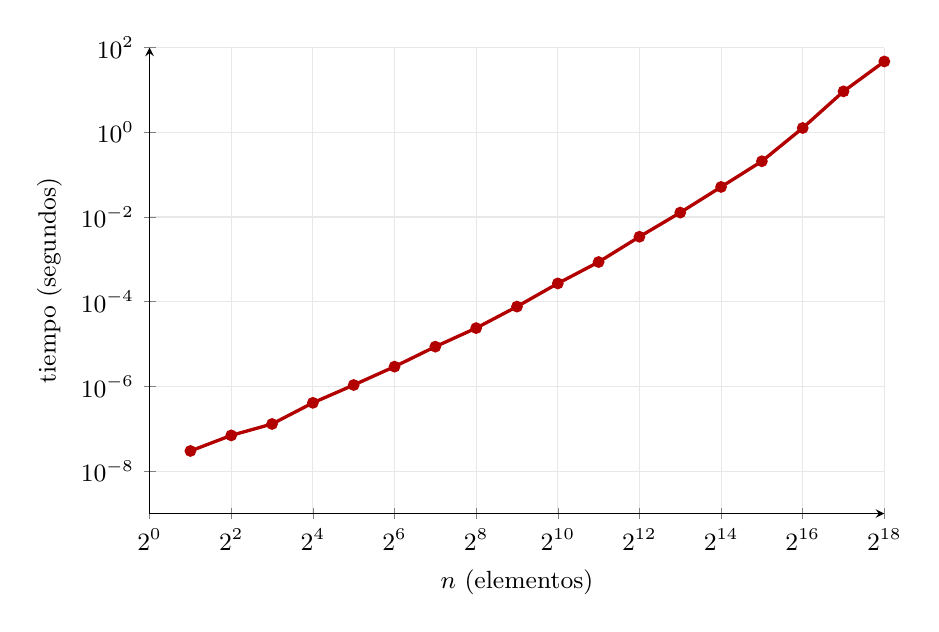
\begin{tikzpicture}
    % Datos medidos con ada/dummy/ComparaOrdenamientos.c
    % (TiemposBurbuja.txt), arreglos aleatorios con semilla fija
    \begin{loglogaxis}[
        width=0.9\linewidth,
        height=7.5cm,
        log basis x=2,
        xmin=1, xmax=262144,
        enlarge x limits=false,
        xtick={1,4,16,64,256,1024,4096,16384,65536,262144},
        xlabel={$n$ (elementos)},
        ylabel={tiempo (segundos)},
        axis lines=left,
        grid=major,
        grid style={gray!18},
        tick label style={font=\small},
        label style={font=\small},
        ymin=1e-9, ymax=1e2,
        ytick={1e-8,1e-6,1e-4,1e-2,1e0,1e2}
      ]
      \addplot[very thick, red!70!black, mark=*, mark size=1.5pt]
        coordinates {
          (2,3.0e-8)           (4,7.0e-8)
          (8,1.3e-7)           (16,4.11e-7)
          (32,1.082e-6)        (64,2.936e-6)
          (128,8.696e-6)       (256,2.3855e-5)
          (512,7.6743e-5)      (1024,2.70035e-4)
          (2048,8.65236e-4)    (4096,3.416622e-3)
          (8192,1.2709973e-2)  (16384,5.1199151e-2)
          (32768,2.0714347e-1) (65536,1.262043866)
          (131072,9.236331467) (262144,46.860850911)
        };
    \end{loglogaxis}
  \end{tikzpicture}
  \caption{Tiempo de bubble sort sobre arreglos aleatorios de $2^1$ a
    $2^{18}$ elementos.}
  \label{fig:tiempos-burbuja}
\end{figure}

Estos datos son discretos, no son continuos pero podemos aproximar una funcion, interpolar, usar alguna tecnica de algoritmos evolutivos o hasta con intuicion

\begin{figure}[htbp]
  \centering
  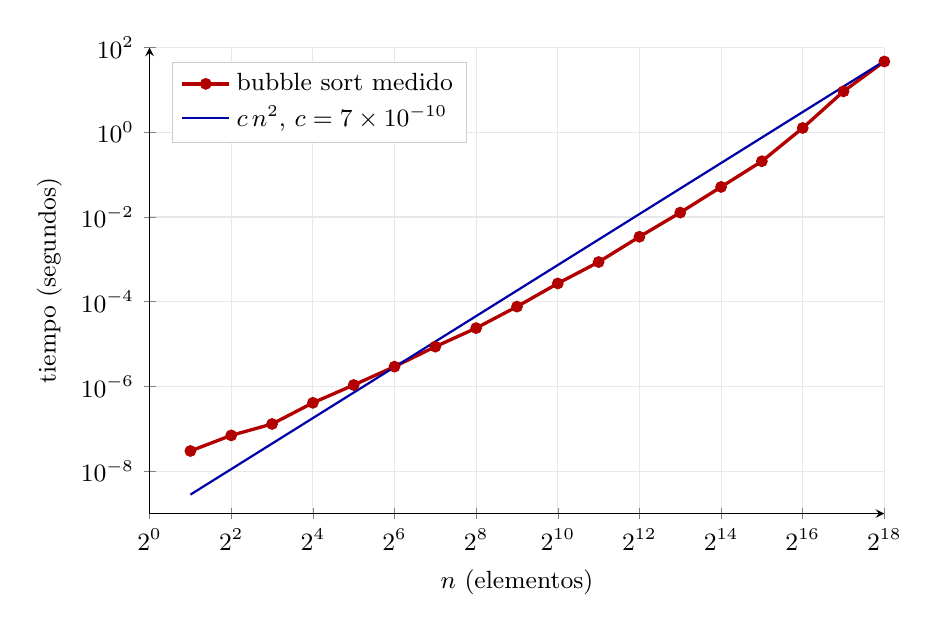
\begin{tikzpicture}
    % Mismos datos de ada/dummy/TiemposBurbuja.txt; la curva roja
    % es c*n^2 con c = 7e-10, ajustada para acotar los puntos
    \begin{loglogaxis}[
        width=0.9\linewidth,
        height=7.5cm,
        log basis x=2,
        xmin=1, xmax=262144,
        enlarge x limits=false,
        xtick={1,4,16,64,256,1024,4096,16384,65536,262144},
        xlabel={$n$ (elementos)},
        ylabel={tiempo (segundos)},
        axis lines=left,
        grid=major,
        grid style={gray!18},
        tick label style={font=\small},
        label style={font=\small},
        ymin=1e-9, ymax=1e2,
        ytick={1e-8,1e-6,1e-4,1e-2,1e0,1e2},
        legend pos=north west,
        legend style={font=\small, draw=gray!40},
        legend cell align=left
      ]
      \addplot[very thick, red!70!black, mark=*, mark size=1.5pt]
        coordinates {
          (2,3.0e-8)           (4,7.0e-8)
          (8,1.3e-7)           (16,4.11e-7)
          (32,1.082e-6)        (64,2.936e-6)
          (128,8.696e-6)       (256,2.3855e-5)
          (512,7.6743e-5)      (1024,2.70035e-4)
          (2048,8.65236e-4)    (4096,3.416622e-3)
          (8192,1.2709973e-2)  (16384,5.1199151e-2)
          (32768,2.0714347e-1) (65536,1.262043866)
          (131072,9.236331467) (262144,46.860850911)
        };
      \addlegendentry{bubble sort medido}
      \addplot[thick, blue!65!black, domain=2:262144, samples=100]
        {7e-10*x^2};
      \addlegendentry{$c\,n^2$, $c = 7 \times 10^{-10}$}
    \end{loglogaxis}
  \end{tikzpicture}
  \caption{Tiempos medidos de bubble sort contra la curva $c\,n^2$.}
  \label{fig:burbuja-cota}
\end{figure}

Se puede ver que la curva $c\,n^2$ está encima de los puntos medidos, así que podemos decir que el tiempo de bubble sort es $\Ord{n^2}$.

\begin{pendiente}
  La curva $c\,n^2$ es una cota superior, pero no es la mejor. ¿Cómo
  encontrar la mejor cota?... LO digo pq como que no acota todos los puntos
  y ademas se ve como una linea recta pero quiza sea por la escala

   UPDATE: No toca los puntos por lo dicho abajo, para valores pequeños es irrelevante, el problema es que no se eligio un buen $n_0$ pero le pregunto al profe.
\end{pendiente}

\subsection*{Quick sort}

Ahora el mismo experimento con quick sort, los datos (resultados) se muestran a continuacion:

\begin{figure}[htbp]
  \centering
  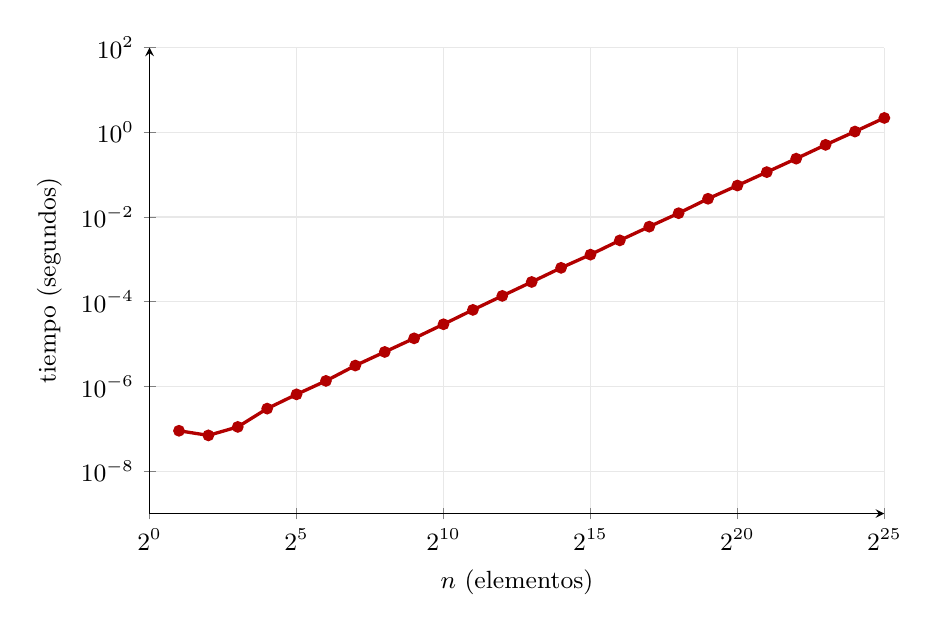
\begin{tikzpicture}
    % Datos medidos con ada/dummy/ComparaOrdenamientos.c
    % (TiemposQuick.txt), mismos arreglos que la burbuja
    \begin{loglogaxis}[
        width=0.9\linewidth,
        height=7.5cm,
        log basis x=2,
        xmin=1, xmax=33554432,
        enlarge x limits=false,
        xtick={1,32,1024,32768,1048576,33554432},
        xlabel={$n$ (elementos)},
        ylabel={tiempo (segundos)},
        axis lines=left,
        grid=major,
        grid style={gray!18},
        tick label style={font=\small},
        label style={font=\small},
        ymin=1e-9, ymax=1e2,
        ytick={1e-8,1e-6,1e-4,1e-2,1e0,1e2}
      ]
      \addplot[very thick, red!70!black, mark=*, mark size=1.5pt]
        coordinates {
          (2,9.0e-8)            (4,7.0e-8)
          (8,1.11e-7)           (16,3.00e-7)
          (32,6.51e-7)          (64,1.353e-6)
          (128,3.116e-6)        (256,6.523e-6)
          (512,1.3666e-5)       (1024,2.9395e-5)
          (2048,6.4190e-5)      (4096,1.37446e-4)
          (8192,2.92677e-4)     (16384,6.30798e-4)
          (32768,1.292354e-3)   (65536,2.807304e-3)
          (131072,5.913627e-3)  (262144,1.2293033e-2)
          (524288,2.6950273e-2) (1048576,5.5287686e-2)
          (2097152,0.114650774) (4194304,0.238225618)
          (8388608,0.504469160) (16777216,1.039287692)
          (33554432,2.178605052)
        };
    \end{loglogaxis}
  \end{tikzpicture}
  \caption{Tiempo de quick sort sobre arreglos aleatorios de $2^1$ a
    $2^{25}$ elementos.}
  \label{fig:tiempos-quick}
\end{figure}

Al tratar de determianr la funcion analitica a ojo de buen cubero...

\begin{figure}[htbp]
  \centering
  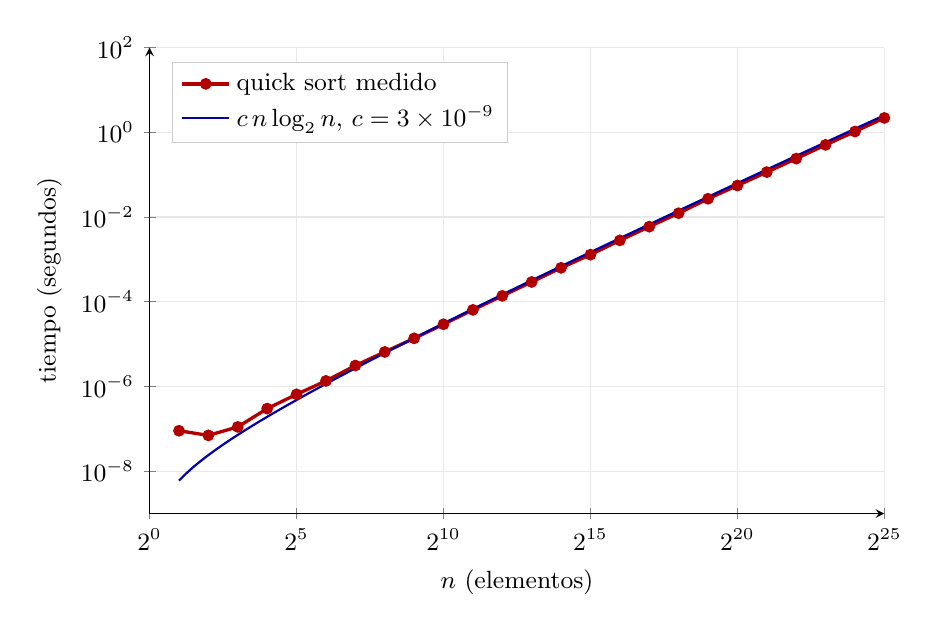
\begin{tikzpicture}
    % La curva roja es c*n*log2(n) con c = 3e-9, ajustada para
    % acotar los puntos medidos
    \begin{loglogaxis}[
        width=0.9\linewidth,
        height=7.5cm,
        log basis x=2,
        xmin=1, xmax=33554432,
        enlarge x limits=false,
        xtick={1,32,1024,32768,1048576,33554432},
        xlabel={$n$ (elementos)},
        ylabel={tiempo (segundos)},
        axis lines=left,
        grid=major,
        grid style={gray!18},
        tick label style={font=\small},
        label style={font=\small},
        ymin=1e-9, ymax=1e2,
        ytick={1e-8,1e-6,1e-4,1e-2,1e0,1e2},
        legend pos=north west,
        legend style={font=\small, draw=gray!40},
        legend cell align=left
      ]
      \addplot[very thick, red!70!black, mark=*, mark size=1.5pt]
        coordinates {
          (2,9.0e-8)            (4,7.0e-8)
          (8,1.11e-7)           (16,3.00e-7)
          (32,6.51e-7)          (64,1.353e-6)
          (128,3.116e-6)        (256,6.523e-6)
          (512,1.3666e-5)       (1024,2.9395e-5)
          (2048,6.4190e-5)      (4096,1.37446e-4)
          (8192,2.92677e-4)     (16384,6.30798e-4)
          (32768,1.292354e-3)   (65536,2.807304e-3)
          (131072,5.913627e-3)  (262144,1.2293033e-2)
          (524288,2.6950273e-2) (1048576,5.5287686e-2)
          (2097152,0.114650774) (4194304,0.238225618)
          (8388608,0.504469160) (16777216,1.039287692)
          (33554432,2.178605052)
        };
      \addlegendentry{quick sort medido}
      \addplot[thick, blue!65!black, domain=2:33554432, samples=100]
        {3e-9*x*ln(x)/ln(2)};
      \addlegendentry{$c\,n\log_2 n$, $c = 3 \times 10^{-9}$}
    \end{loglogaxis}
  \end{tikzpicture}
  \caption{Tiempos medidos de quick sort contra la curva
    $c\,n\log_2 n$.}
  \label{fig:quick-cota}
\end{figure}

\newpage

La curva $c\,n\log_2 n$ acota mas o menos bien los puntos medidos, asi que podemos decir que el tiempo de quick sort es $\Ord{n \log n}$.

\begin{pendiente}
  Igual que en burbuja, por que no acota todos los puntos??

  UPDATE: No toca los puntos por lo dicho abajo, para valores pequeños es irrelevante, el problema es que no se eligio un buen $n_0$ pero le pregunto al profe.
\end{pendiente}

\newpage

\subsection*{Brubuja vs Quick}
Al comparar ambos algoritmos en la sig grafica...

\begin{figure}[htbp]
  \centering
  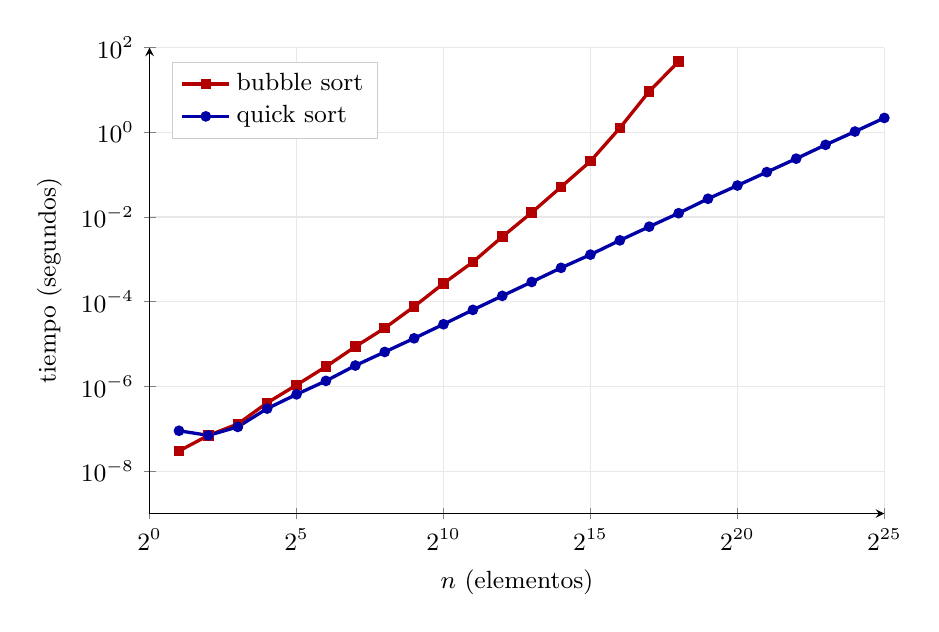
\begin{tikzpicture}
    % Las dos series salen de la misma corrida de
    % ada/dummy/ComparaOrdenamientos.c, sobre los mismos arreglos
    \begin{loglogaxis}[
        width=0.9\linewidth,
        height=7.5cm,
        log basis x=2,
        xlabel={$n$ (elementos)},
        ylabel={tiempo (segundos)},
        axis lines=left,
        grid=major,
        grid style={gray!18},
        tick label style={font=\small},
        label style={font=\small},
        xmin=1, xmax=33554432,
        enlarge x limits=false,
        xtick={1,32,1024,32768,1048576,33554432},
        ymin=1e-9, ymax=1e2,
        ytick={1e-8,1e-6,1e-4,1e-2,1e0,1e2},
        legend pos=north west,
        legend style={font=\small, draw=gray!40},
        legend cell align=left
      ]
      \addplot[very thick, red!70!black, mark=square*, mark size=1.3pt]
        coordinates {
          (2,3.0e-8)           (4,7.0e-8)
          (8,1.3e-7)           (16,4.11e-7)
          (32,1.082e-6)        (64,2.936e-6)
          (128,8.696e-6)       (256,2.3855e-5)
          (512,7.6743e-5)      (1024,2.70035e-4)
          (2048,8.65236e-4)    (4096,3.416622e-3)
          (8192,1.2709973e-2)  (16384,5.1199151e-2)
          (32768,2.0714347e-1) (65536,1.262043866)
          (131072,9.236331467) (262144,46.860850911)
        };
      \addlegendentry{bubble sort}
      \addplot[very thick, blue!65!black, mark=*, mark size=1.3pt]
        coordinates {
          (2,9.0e-8)            (4,7.0e-8)
          (8,1.11e-7)           (16,3.00e-7)
          (32,6.51e-7)          (64,1.353e-6)
          (128,3.116e-6)        (256,6.523e-6)
          (512,1.3666e-5)       (1024,2.9395e-5)
          (2048,6.4190e-5)      (4096,1.37446e-4)
          (8192,2.92677e-4)     (16384,6.30798e-4)
          (32768,1.292354e-3)   (65536,2.807304e-3)
          (131072,5.913627e-3)  (262144,1.2293033e-2)
          (524288,2.6950273e-2) (1048576,5.5287686e-2)
          (2097152,0.114650774) (4194304,0.238225618)
          (8388608,0.504469160) (16777216,1.039287692)
          (33554432,2.178605052)
        };
      \addlegendentry{quick sort}
    \end{loglogaxis}
  \end{tikzpicture}
  \caption{Bubble sort contra quick sort sobre los mismos arreglos.
    segundos.}
  \label{fig:burbuja-vs-quick}
\end{figure}

Se puede ver que quick sort es mucho mas rapido que burbuja, y la diferencia se hace mas evidente a medida que el tamaño del arreglo crece. Por ejemplo, burbuja lo detuve en $2^{18}$ elementos porque ya tardaba demasiado, mientras que quick sort lo corrí hasta $2^{25}$ elementos y seguía siendo razonable.
Entonces podemos concluir que quick sort es mucho mas eficiente que burbuja.

\begin{ojo}
  Se puede hacer esta comparacion ya que los arreglos que se usan para probar ambos algoritmos fueron los mismos y se testeo en la misma PC. 
  El codigo se encuentra en https://github.com/zxxz456/inaoe/tree/main/ada/dummy/ComparaOrdenamientos.c
\end{ojo}

\newpage

\subsection*{Notacion Big O}
En los ejemplos de arriba mencione que el tiempo de bubble sort es $\Ord{n^2}$ y el tiempo de quick sort es $\Ord{n \log n}$.

Lo que quiere decir esto es que la funcion empirica encontrada del ALGORITMO de ordenamiento burbuja $f(n)$, pertenece al conjunto de funciones o a la familia de funciones $\Ord{n^2}$

Y analogamente la funcion empirica encontrada del ALGORITMO de ordenamiento quick sort $f(n)$, pertenece al conjunto de funciones o a la familia de funciones $\Ord{n \log n}$

De forma mas general, nuestra funcion empirica $f(n)$ la queremos modelar como una funcion continua $c \cdot g(n)$
y dada esta funcion $g(n)$ denotamos $\Ord{g(n)}$ al conjunto de funciones tales que existen constntes positivas
$c$ y $n_0$ tales que para todo $n \geq n_0$ se cumple que $f(n) \leq c \cdot g(n)$

\begin{definicion}
  Sea $g(n)$ una función positiva. Decimos que una función $f(n)$ pertenece a
  $\Ord{g(n)}$ si existen constantes positivas $c$ y $n_0$ tales que
  \[
    0 \leq f(n) \leq c \cdot g(n) \qquad \text{para todo } n \geq n_0 .
  \]
  Equivalentemente,
  \[
    \Ord{g(n)} = \{\, f(n) : \exists\, c > 0,\; \exists\, n_0 > 0
    \ \text{tales que}\ 0 \leq f(n) \leq c\cdot g(n)\ \ \forall\, n \geq n_0 \,\}.
  \]
\end{definicion}

Y lo que dice basicamente es que $f(n)$ esta en el conjunto de funciones $\Ord{g(n)}$ y que crece a lo mucho como esa $g(n)$

\begin{ejemplo}
  Sean $f(n) = 2n^{2} + 3n + 1$ y $g(n) = n^{2}$. Tomando $c = 6$ y $n_0 = 1$
  se cumple
  \[
    2n^{2} + 3n + 1 \;\leq\; 6n^{2}
    \iff 4n^{2} - 3n - 1 \geq 0
    \iff (4n + 1)(n - 1) \geq 0,
  \]
  lo cual es cierto para todo $n \geq 1$. Por lo tanto $f(n) \in \Ord{n^{2}}$.

  El par $(c, n_0)$ no es único: con $c = 3$ la desigualdad
  $2n^{2} + 3n + 1 \leq 3n^{2}$ equivale a $n^{2} - 3n - 1 \geq 0$, que se
  satisface a partir de $n \geq \tfrac{3 + \sqrt{13}}{2} \approx 3.30$, de modo
  que $n_0 = 4$ también funciona. La definición solo exige que \emph{exista}
  al menos un par de constantes.
\end{ejemplo}


\begin{figure}[htbp]
  \centering
  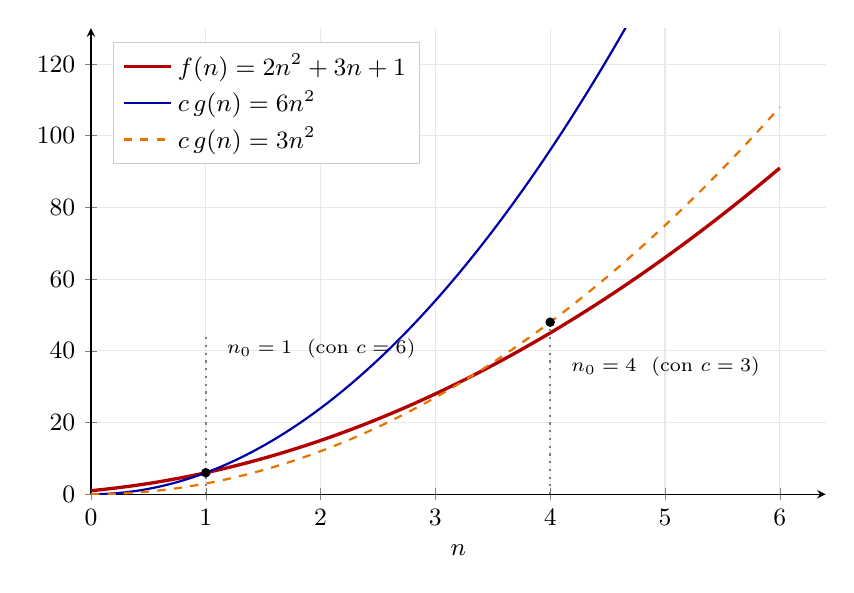
\begin{tikzpicture}
    \begin{axis}[
      width=0.9\linewidth, height=7.5cm,
      xlabel={$n$},
      domain=0:6, samples=200,
      xmin=0, xmax=6.4, ymin=0, ymax=130,
      axis lines=left,
      legend pos=north west,
      legend cell align=left,
      grid=major, grid style={gray!18},
      tick label style={font=\small},
      label style={font=\small},
      legend style={font=\small, draw=gray!40},
      xtick={0,1,2,3,4,5,6},
    ]
      \addplot[very thick, red!70!black] {2*x^2+3*x+1};
      \addlegendentry{$f(n)=2n^{2}+3n+1$}
      \addplot[thick, blue!65!black] {6*x^2};
      \addlegendentry{$c\,g(n)=6n^{2}$}
      \addplot[thick, orange!90!black, dashed] {3*x^2};
      \addlegendentry{$c\,g(n)=3n^{2}$}
      \draw[gray, dotted, thick] (axis cs:1,0) -- (axis cs:1,45);
      \draw[gray, dotted, thick] (axis cs:4,0) -- (axis cs:4,48);
      \node[anchor=north west, font=\scriptsize] at (axis cs:1.1,46)
        {$n_0=1$ \ (con $c=6$)};
      \node[anchor=north west, font=\scriptsize] at (axis cs:4.1,41)
        {$n_0=4$ \ (con $c=3$)};
      \addplot[only marks, mark=*, mark size=1.5pt, black]
        coordinates {(1,6) (4,48)};
    \end{axis}
  \end{tikzpicture}
  \caption{Para $n \geq 1$ la curva $6n^{2}$ domina a $f(n)$; a partir de
  $n \geq 4$ basta con $3n^{2}$.}
  \label{fig:big-o-ejemplo}
\end{figure}

\newpage

\begin{ojo}
  El "para todo $n \geq n_0$" es lo que hace que la def sea asintotica. El comportamiento en entradas
  chiquitas es irrelevante, la curva $f$ puede estar por encima de $c g(n)$ tanto como sea antes del umbral.
\end{ojo}

\vspace{2em}

\begin{ojo}
  La Big O da una cota superior q no tiene que ser ajustada. Es
  perfectamente cierto que $n = \Ord{n^5}$, aunque sea una cota muy
  floja. Cuando quieres afirmar que la cota es ajustada por arriba y
  por abajo, usas $\Theta(g(n))$, definida con dos constantes:
  $0 \leq c_1 \cdot g(n) \leq f(n) \leq c_2 \cdot g(n)$.
\end{ojo}

\vspace{2em}

\begin{ojo}
  Como $\Ord{g(n)}$ es un conjunto, lo correcto sería escribir
  $f(n) \in \Ord{g(n)}$. La costumbre de escribir $f(n) = \Ord{g(n)}$
  es un abuso de notación establecido, y por eso el signo no es
  simétrico: puedes escribir $2n^2 = \Ord{n^3}$, pero nunca
  $\Ord{n^3} = 2n^2$.
\end{ojo}

\subsection*{Crecimiento de funciones}

Determinar la eficiencia asintótica de un algoritmo pasa por
modelarlo: encontrar la función que describe su costo y ver contra
qué se puede acotar. Muchas funciones admiten cota asintótica, y en
la práctica casi todo termina comparándose contra tres familias:
polinomios, logaritmos y exponenciales.

\subsubsection*{Operación elemental}

\begin{definicion}
  Una operación elemental es aquella cuyo tiempo de ejecución está
  acotado por una constante que no depende del tamaño de la entrada.
  Una comparación, una asignación o una suma cuentan como una sola,
  sin importar qué tan grande sea $n$
\end{definicion}

Un algoritmo casi nunca ejecuta un solo tipo de operación. Sumar dos
matrices de $n \times n$ hace sumas, pero también compara índices,
incrementa contadores y accede a memoria. Se escoge una operación
representativa, la que se ejecuta al menos tan seguido como
cualquier otra, y se cuenta esa nada más: las demás quedan
absorbidas por un factor constante

\subsubsection*{Principio de invarianza}

Dos implementaciones del mismo algoritmo, en lenguajes distintos o
sobre máquinas distintas, no tardan lo mismo, pero sus tiempos
difieren a lo mucho por un factor constante. Esa es la razón de que
la constante se descarte: lo que cambia al cambiar de máquina es
ella, mientras que la clase asintótica es propiedad del algoritmo y
sobrevive al cambio

\subsubsection*{Mejor caso, peor caso y caso promedio}

El costo no depende solo de $n$, también de cómo venga la entrada,
así que se analizan tres escenarios. Quick sort es el ejemplo de la
tabla \ref{tab:ordenamiento}: en promedio cuesta $\Ord{n \log n}$,
pero si el pivote cae siempre en un extremo las particiones quedan
desbalanceadas y degenera a $\Ord{n^2}$. La burbuja simple no
distingue, sus tres casos son $\Ord{n^2}$ porque recorre los ciclos
completos sin importar cómo venga el arreglo

\begin{idea}
  Siempre conviene optimizar. Es la única forma de llegar a los
  límites de lo que las arquitecturas actuales pueden dar
\end{idea}

\vspace{2em}




\newpage

% =====================================================================
%  Clase 3 - Omega, Theta y ordenes de complejidad
% =====================================================================

\clase{Continuación de funciones asintóticas}{25 de agosto de 2026}

\begin{quick_sum}
    Continuación de la clase anterior. Las propiedades de las tres
    notaciones, con la regla del límite que las decide de un jalón.
    $\Omg{\cdot}$ como cota inferior, $\Tht{\cdot}$ como las dos a la
    vez y el teorema que las relaciona. Cerramos con las notaciones
    chicas, los órdenes de complejidad y los consejos para contar
    operaciones elementales.
\end{quick_sum}

\subsection*{Propiedades de $\Ord{\cdot}$}

Sean $f$, $g$, $h$, $f_1$ y $f_2$ funciones positivas.

\begin{enumerate}[itemsep=0.15em]
    \item Para cualquier función $f$ se tiene $f \in \Ord{f}$.
    \item $f \in \Ord{g} \Rightarrow \Ord{f} \subset \Ord{g}$.
    \item $\Ord{f} = \Ord{g} \iff f \in \Ord{g}$ y $g \in \Ord{f}$.
    \item Si $f \in \Ord{g}$ y $g \in \Ord{h} \Rightarrow
          f \in \Ord{h}$.
    \item Si $f \in \Ord{g}$ y $f \in \Ord{h} \Rightarrow
          f \in \Ord{\min(g,h)}$.
    \item \textbf{Regla de la suma:} si $f_1 \in \Ord{g}$ y
          $f_2 \in \Ord{h} \Rightarrow
          f_1 + f_2 \in \Ord{\max(g,h)}$.
    \item \textbf{Regla del producto:} si $f_1 \in \Ord{g}$ y
          $f_2 \in \Ord{h} \Rightarrow
          f_1 \cdot f_2 \in \Ord{g \cdot h}$.
    \item Si existe $\displaystyle\lim_{n \to \infty} \frac{f(n)}{g(n)}
          = k$, entonces según el valor de $k$:
          \begin{itemize}[itemsep=0.05em]
              \item Si $k \neq 0$ y $k < \infty$, entonces
                    $\Ord{f} = \Ord{g}$.
              \item Si $k = 0$, entonces $f \in \Ord{g}$, es decir
                    $\Ord{f} \subset \Ord{g}$, pero se verifica que
                    $g \notin \Ord{f}$.
          \end{itemize}
\end{enumerate}

\begin{idea}
    La propiedad del límite es la herramienta práctica. En lugar de
    buscar $c$ y $n_0$ a mano, se calcula el cociente $f/g$ y se ve a
    dónde tiende: si tiende a una constante distinta de cero, las dos
    funciones son del mismo orden; si tiende a cero, $f$ crece
    estrictamente más despacio.
\end{idea}

% =====================================================================

\subsection*{Notación Omega}

$f(n) = \Omg{g(n)}$ quiere decir que $g(n)$ es una cota asintótica
inferior de $f(n)$.

\begin{definicion}
  Sea $g(n)$ una función positiva. Decimos que una función $f(n)$
  pertenece a $\Omg{g(n)}$ si existen constantes positivas $c$ y $n_0$
  tales que
  \[
    0 \leq c \cdot g(n) \leq f(n) \qquad \text{para todo } n \geq n_0 .
  \]
  Equivalentemente,
  \[
    \Omg{g(n)} = \{\, f(n) : \exists\, c > 0,\; \exists\, n_0 > 0
    \ \text{tales que}\ 0 \leq c \cdot g(n) \leq f(n)
    \ \ \forall\, n \geq n_0 \,\}.
  \]
\end{definicion}

\begin{ojo}
    $f(n) \in \Omg{g(n)}$ si y solo si $g(n) \in \Ord{f(n)}$. Las dos
    notaciones son la misma relación vista desde cada lado.
\end{ojo}

\subsubsection*{Propiedades de $\Omg{\cdot}$}

\begin{enumerate}[itemsep=0.15em]
    \item Para cualquier función $f$ se tiene $f \in \Omg{f}$.
    \item $f \in \Omg{g} \Rightarrow \Omg{f} \subset \Omg{g}$.
    \item $\Omg{f} = \Omg{g} \iff f \in \Omg{g}$ y $g \in \Omg{f}$.
    \item Si $f \in \Omg{g}$ y $g \in \Omg{h} \Rightarrow
          f \in \Omg{h}$.
    \item Si $f \in \Omg{g}$ y $f \in \Omg{h} \Rightarrow
          f \in \Omg{\max(g,h)}$.
    \item \textbf{Regla de la suma:} si $f_1 \in \Omg{g}$ y
          $f_2 \in \Omg{h} \Rightarrow f_1 + f_2 \in \Omg{g + h}$.
    \item \textbf{Regla del producto:} si $f_1 \in \Omg{g}$ y
          $f_2 \in \Omg{h} \Rightarrow
          f_1 \cdot f_2 \in \Omg{g \cdot h}$.
    \item Si existe $\displaystyle\lim_{n \to \infty} \frac{f(n)}{g(n)}
          = k$, entonces según el valor de $k$:
          \begin{itemize}[itemsep=0.05em]
              \item Si $k \neq 0$ y $k < \infty$, entonces
                    $\Omg{f} = \Omg{g}$.
              \item Si $k = 0$, entonces $g \in \Omg{f}$, es decir
                    $\Omg{g} \subset \Omg{f}$, pero se verifica que
                    $f \notin \Omg{g}$.
          \end{itemize}
\end{enumerate}

\begin{ojo}
    En $\Ord{\cdot}$ la propiedad 5 usa el mínimo y la regla de la
    suma el máximo. En $\Omg{\cdot}$ la 5 usa el máximo y la suma da
    $g + h$. No son simétricas, conviene no copiarlas de memoria.
\end{ojo}

\subsubsection*{Por qué importan las cotas inferiores}

Una cota inferior dice cuándo ya no se puede mejorar dentro de un
modelo de cómputo. El ejemplo canónico es el ordenamiento por
comparaciones: en el modelo general de comparaciones, cualquier
algoritmo de ordenamiento necesita del orden de $n \log n$
comparaciones en el peor caso, o sea $\Omg{n \log n}$.

\begin{idea}
    Si un algoritmo ya logra $\Ord{n \log n}$ y el problema tiene cota
    inferior $\Omg{n \log n}$, entonces ese algoritmo es
    asintóticamente óptimo en ese modelo. $\Omg{\cdot}$ contesta cuál
    es el trabajo mínimo que hay que hacer.
\end{idea}

% =====================================================================

\subsection*{Notación Theta}

$f(n) = \Tht{g(n)}$ quiere decir que $c_2\,g(n)$ y $c_1\,g(n)$ son las
cotas asintóticas de $f(n)$, superior e inferior respectivamente.
Diremos que $f(n) \in \Tht{g(n)}$ si $f(n)$ pertenece tanto a
$\Ord{g(n)}$ como a $\Omg{g(n)}$.

\begin{definicion}
  Sea $g(n)$ una función positiva. Decimos que una función $f(n)$
  pertenece a $\Tht{g(n)}$ si existen constantes positivas $c_1$,
  $c_2$ y $n_0$ tales que
  \[
    0 < c_1 \cdot g(n) \leq f(n) \leq c_2 \cdot g(n)
    \qquad \text{para todo } n \geq n_0 .
  \]
  Equivalentemente,
  \[
    \Tht{g(n)} = \{\, f(n) : \exists\, c_1 > 0,\; \exists\, c_2 > 0,\;
    \exists\, n_0 > 0 \ \text{tales que}\
    0 < c_1 \cdot g(n) \leq f(n) \leq c_2 \cdot g(n)
    \ \ \forall\, n \geq n_0 \,\}.
  \]
\end{definicion}

\subsubsection*{Propiedades de $\Tht{\cdot}$}

\begin{enumerate}[itemsep=0.15em]
    \item Para cualquier función $f$ se tiene $f \in \Tht{f}$.
    \item $f \in \Tht{g} \Rightarrow \Tht{f} \subset \Tht{g}$.
    \item $\Tht{f} = \Tht{g} \iff f \in \Tht{g}$ y $g \in \Tht{f}$.
    \item Si $f \in \Tht{g}$ y $g \in \Tht{h} \Rightarrow
          f \in \Tht{h}$.
    \item \textbf{Regla de la suma:} si $f_1 \in \Tht{g}$ y
          $f_2 \in \Tht{h} \Rightarrow
          f_1 + f_2 \in \Tht{\max(g,h)}$.
    \item \textbf{Regla del producto:} si $f_1 \in \Tht{g}$ y
          $f_2 \in \Tht{h} \Rightarrow
          f_1 \cdot f_2 \in \Tht{g \cdot h}$.
    \item Si existe $\displaystyle\lim_{n \to \infty} \frac{f(n)}{g(n)}
          = k$, entonces según el valor de $k$:
          \begin{itemize}[itemsep=0.05em]
              \item Si $k \neq 0$ y $k < \infty$, entonces
                    $\Tht{f} = \Tht{g}$.
              \item Si $k = 0$, entonces los órdenes exactos de $f$ y
                    $g$ son distintos.
          \end{itemize}
\end{enumerate}

\begin{teorema}
    $f(n) = \Tht{g(n)}$ si y solo si $f(n) = \Ord{g(n)}$ y
    $f(n) = \Omg{g(n)}$.
\end{teorema}

\begin{proof}
    De ida es inmediato: la definición de $\Tht{\cdot}$ contiene las
    dos desigualdades, así que $c_2$ y $n_0$ sirven de testigo para
    $\Ord{\cdot}$, y $c_1$ y $n_0$ para $\Omg{\cdot}$.

    De regreso, si $f \in \Ord{g}$ existen $c_2$ y $n_1$ con
    $f(n) \leq c_2\,g(n)$ para $n \geq n_1$, y si $f \in \Omg{g}$
    existen $c_1$ y $n_2$ con $c_1\,g(n) \leq f(n)$ para $n \geq n_2$.
    Tomando $n_0 = \max\{n_1, n_2\}$ las dos valen a la vez a partir
    de $n_0$, que es justo la definición de $\Tht{g(n)}$. \qedhere
\end{proof}

% =====================================================================

\subsection*{Una cota puede ser correcta y a la vez imprecisa}

Sea $T(n) = 3n^2 + 7n + 20$. Todas estas afirmaciones son
matemáticamente ciertas:
\[
    T(n) \in \Ord{n^2}, \quad
    T(n) \in \Ord{n^3}, \quad
    T(n) \in \Ord{n^4}, \quad
    T(n) \in \Ord{2^n} .
\]

Cada una de esas funciones se puede escalar por alguna constante
positiva de modo que termine quedando por encima de $T(n)$. Por eso
Big O por sí sola no identifica la verdadera tasa de crecimiento.
$\Tht{n^2}$ sí: dice que el crecimiento cuadrático es el orden
asintótico correcto, salvo factores constantes.

\begin{ojo}
    $\Ord{\cdot}$ no es sinónimo de peor caso, ni $\Omg{\cdot}$ de
    mejor caso. Son relaciones matemáticas de acotamiento. Primero se
    elige qué función de tiempo se está analizando y después se le
    aplica la notación que sea. Se puede decir
    $T_{\text{mejor}}(n) = \Tht{n}$, o
    $T_{\text{peor}}(n) = \Omg{n \log n}$, sin ninguna contradicción.
\end{ojo}

% =====================================================================

\subsection*{Notaciones chicas}

$f(n) = \ord{g(n)}$ quiere decir que $g(n)$ es una cota superior de
$f(n)$ que no es asintóticamente justa (\textit{tight}). Y
$f(n) = \omg{g(n)}$, que $g(n)$ es una cota inferior de $f(n)$ que
tampoco lo es.

\begin{definicion}
  Sea $g(n)$ una función positiva. Decimos que una función $f(n)$
  pertenece a $\ord{g(n)}$ si para toda constante positiva $c$ existe
  $n_0 > 0$ tal que
  \[
    0 \leq f(n) < c \cdot g(n) \qquad \text{para todo } n \geq n_0 .
  \]
  Equivalentemente,
  \[
    \ord{g(n)} = \{\, f(n) : \forall\, c > 0,\; \exists\, n_0 > 0
    \ \text{tales que}\ 0 \leq f(n) < c \cdot g(n)
    \ \ \forall\, n \geq n_0 \,\}.
  \]
\end{definicion}

\begin{definicion}
  Sea $g(n)$ una función positiva. Decimos que una función $f(n)$
  pertenece a $\omg{g(n)}$ si para toda constante positiva $c$ existe
  $n_0 > 0$ tal que
  \[
    0 \leq c \cdot g(n) < f(n) \qquad \text{para todo } n \geq n_0 .
  \]
  Equivalentemente,
  \[
    \omg{g(n)} = \{\, f(n) : \forall\, c > 0,\; \exists\, n_0 > 0
    \ \text{tales que}\ 0 \leq c \cdot g(n) < f(n)
    \ \ \forall\, n \geq n_0 \,\}.
  \]
\end{definicion}

La distinción precisa no es tanto lo justo o no justo, sino el
cuantificador sobre la constante:

\begin{itemize}[itemsep=0.3em]
    \item $f(n) = \Ord{g(n)} \iff \exists\, c > 0,\ \exists\, n_0 :\;
          f(n) \leq c\,g(n),\ \forall\, n \geq n_0$.
    \item $f(n) = \ord{g(n)} \iff \forall\, c > 0,\ \exists\, n_0 :\;
          f(n) < c\,g(n),\ \forall\, n \geq n_0$.
\end{itemize}

Con $\Omg{\cdot}$ y $\omg{\cdot}$ pasa lo mismo, volteando la
desigualdad. Las grandes permiten que las dos funciones sean del
mismo orden; las chicas lo prohíben.

\begin{table}[htbp]
  \centering
  \small
  \begin{tabular}{lll}
    \toprule
    \textbf{Propiedad} & $\Ord{g(n)}$ & $\ord{g(n)}$ \\
    \midrule
    Tipo de cota superior      & No estricta & Estricta \\
    Condición sobre $c$        & $\exists\, c > 0$ & $\forall\, c > 0$ \\
    Permite el mismo orden     & Sí & No \\
    Puede ser $\Tht{g(n)}$     & Sí & No \\
    Cociente $f(n)/g(n)$       & Acotado basta & Tiende a $0$ \\
    \bottomrule
  \end{tabular}
  \caption{Big O contra o chica.}
  \label{tab:o-chica}
\end{table}

\subsubsection*{El punto de vista del límite}

Cuando el límite existe, el cociente deja la distinción clarísima:
\[
    f = \ord{g} \iff \frac{f(n)}{g(n)} \to 0, \qquad
    f = \Tht{g} \iff \frac{f(n)}{g(n)} \to L \text{ con }
    0 < L < \infty, \qquad
    f = \omg{g} \iff \frac{f(n)}{g(n)} \to \infty .
\]

$\Ord{\cdot}$ y $\Omg{\cdot}$ son relaciones más amplias: solo piden
una cota por factor constante, no un límite específico. Por ejemplo
$n^2 \neq \ord{n^2}$, porque el cociente vale $1$ y no $0$; en cambio
$n = \ord{n^2}$, porque $n/n^2 = 1/n \to 0$.

\subsubsection*{Jerarquía de crecimiento}

\[
    1 \ll \log n \ll n \ll n \log n \ll n^2 \ll n^3 \ll 2^n
\]

Leída con o chica: $n = \ord{n \log n}$,
$n \log n = \ord{n^2}$, $n^2 = \ord{n^3}$. Y al revés con omega
chica: $n \log n = \omg{n}$, $n^2 = \omg{n \log n}$,
$n^3 = \omg{n^2}$.

\begin{table}[htbp]
  \centering
  \small
  \begin{tabular}{lll}
    \toprule
    \textbf{Notación} & \textbf{Crecimiento} & \textbf{Tipo de cota} \\
    \midrule
    $\ord{g(n)}$   & Estrictamente más lento  & Superior estricta \\
    $\Ord{g(n)}$   & No más rápido            & Superior \\
    $\Tht{g(n)}$   & Del mismo orden          & Ajustada \\
    $\Omg{g(n)}$   & No más lento             & Inferior \\
    $\omg{g(n)}$   & Estrictamente más rápido & Inferior estricta \\
    \bottomrule
  \end{tabular}
  \caption{Las cinco relaciones asintóticas de un vistazo.}
  \label{tab:cinco}
\end{table}

\begin{idea}
    $\ord{\cdot} < \Ord{\cdot} - \Tht{\cdot} - \Omg{\cdot} <
    \omg{\cdot}$. Las grandes admiten crecimiento del mismo orden,
    las chicas lo prohíben. Esa es toda la diferencia.
\end{idea}

% =====================================================================

\subsection*{Orden de complejidad}

La familia $\Ord{f(n)}$, $\Omg{f(n)}$, $\Tht{f(n)}$ define un orden de
complejidad, y como representante del orden se elige la función $f(n)$
más sencilla de la familia. Se identifican diferentes familias:

\begin{table}[htbp]
  \centering
  \begin{tabular}{ll}
    \toprule
    \textbf{Orden} & \textbf{Nombre} \\
    \midrule
    $\Ord{c}$          & Constante \\
    $\Ord{\log n}$     & Logarítmico \\
    $\Ord{n}$          & Lineal \\
    $\Ord{n \log n}$   & Casi lineal \\
    $\Ord{n^2}$        & Cuadrático \\
    $\Ord{n^3}$        & Cúbico \\
    $\Ord{n^c}$        & Polinómico de grado $c$ \\
    $\Ord{2^n}$        & Exponencial \\
    $\Ord{n!}$         & Factorial \\
    \bottomrule
  \end{tabular}
  \caption{Órdenes de complejidad.}
  \label{tab:ordenes}
\end{table}

% =====================================================================

\subsection*{Consejos para identificar $f(n)$}

Son los consejos para dar con la $f(n)$ que representa el número de
operaciones elementales (OE) de un algoritmo.

\subsubsection*{Consejo 1: la base}

Se asume que el tiempo de una OE es de orden $1$, o sea que la
constante $c$ del principio de invarianza se toma como $1$ por fines
prácticos. El tiempo de ejecución de una secuencia de instrucciones,
elementales o no, se obtiene sumando los tiempos de cada instrucción.

\subsubsection*{Instrucción \texttt{case}}

Para \texttt{switch(n)} con casos $S_1, \dots, S_k$:
\[
    f(n) = f(c) + \max\{f(S_1), \dots, f(S_k)\} ,
\]
donde $f(c)$ considera el tiempo de comparar $n$ contra cada uno de
los casos.

\subsubsection*{Instrucción \texttt{if}}

Para \texttt{if C then} $S_1$ \texttt{else} $S_2$:
\[
    f(n) = f(C) + \max\{f(S_1), f(S_2)\} .
\]

\begin{lstlisting}[language=C]
if (n == 0)
    for (i = 0; i < n; i++)
        r += i;
else
    r = 2;
\end{lstlisting}

\subsubsection*{Instrucción \texttt{while}}

Para \texttt{while (c) \{ S \}}:
\[
    f(n) = f(c) + (\text{\#iteraciones}) \cdot (f(c) + f(S)) .
\]

\begin{ojo}
    Las instrucciones \texttt{for}, \texttt{repeat} y \texttt{loop}
    son equivalentes a un \texttt{while}, así que se analizan con la
    misma fórmula.
\end{ojo}

\subsubsection*{Llamado a funciones no recursivas}

El tiempo de una llamada $F(A_1, \dots, A_s)$ es $1$ por el llamado,
más el tiempo de evaluar los parámetros, más el tiempo de ejecutar el
cuerpo de la función:
\[
    f(A_1, \dots, A_s) = 1 + f(A_1) + \cdots + f(A_s) + f(S) .
\]

\subsubsection*{Funciones recursivas}

El tiempo de ejecución de una función recursiva se calcula a través de
la solución de funciones de recurrencia, que es el tema que sigue.

\newpage

% =====================================================================
%  Anexo - Caracterizacion por limites
% =====================================================================

\section{Anexo: caracterización por límites}

Herramienta de diagnóstico para $\Ord{\cdot}$, $\Omg{\cdot}$,
$\Tht{\cdot}$, $\ord{\cdot}$ y $\omg{\cdot}$.

\subsection*{La idea que hay detrás}

Todas estas notaciones comparan el tamaño de dos funciones, y la
manera natural de comparar tamaños es dividir. Si $f$ y $g$ son
positivas para $n$ suficientemente grande, toda la información
relevante está en el cociente $f(n)/g(n)$.

\begin{idea}[title={Traducción de cada notación al cociente}]
    $f \in \Ord{g}$ significa que el cociente está \emph{acotado por
    arriba} en la cola. $f \in \Omg{g}$ significa que está
    \emph{acotado lejos de cero}. $f \in \Tht{g}$ significa ambas
    cosas. Las versiones minúsculas son las variantes estrictas:
    $\ord{\cdot}$ pide que el cociente \emph{colapse} a cero, y
    $\omg{\cdot}$ que \emph{explote} a infinito.
\end{idea}

Conviene ver por qué la definición de $\Ord{\cdot}$ es exactamente un
enunciado de acotación. La condición $f(n) \leq c\,g(n)$ para todo
$n \geq n_0$ equivale, dividiendo entre $g(n) > 0$, a
$f(n)/g(n) \leq c$ para todo $n \geq n_0$. Es decir: la constante $c$
de la definición es literalmente una cota superior del cociente, y el
umbral $n_0$ es el permiso para ignorar un tramo inicial finito. Esa
lectura es la que hace transparente todo lo demás.

% =====================================================================

\subsection*{Criterio con el límite ordinario}

Este es el caso cómodo y cubre la gran mayoría de los ejercicios,
porque polinomios, logaritmos y exponenciales son funciones bien
portadas cuyos cocientes convergen.

Supóngase que existe
\[
    L \;=\; \LM \frac{f(n)}{g(n)}
\]
admitiendo el valor $+\infty$. Entonces se tiene la clasificación
siguiente.

\begin{table}[htbp]
  \centering
  \begin{tabular}{@{}lll@{}}
    \toprule
    \textbf{Valor de $L$} & \textbf{Relación más fuerte}
      & \textbf{Relaciones implicadas} \\
    \midrule
    $L = 0$          & $f \in \ord{g}$ & $f \in \Ord{g}$ \\
    $0 < L < \infty$ & $f \in \Tht{g}$
      & $f \in \Ord{g}$ y $f \in \Omg{g}$ \\
    $L = \infty$     & $f \in \omg{g}$ & $f \in \Omg{g}$ \\
    \bottomrule
  \end{tabular}
  \caption{Clasificación según el límite del cociente.}
  \label{tab:criterio-limite}
\end{table}

En el primer renglón fallan $\Omg{\cdot}$, $\Tht{\cdot}$ y
$\omg{\cdot}$. En el segundo fallan $\ord{\cdot}$ y $\omg{\cdot}$. En
el tercero fallan $\Ord{\cdot}$, $\Tht{\cdot}$ y $\ord{\cdot}$. Y si
el límite no existe, el criterio no dice nada y hay que pasar a la
sección siguiente.

\begin{observacion}
    El primer renglón es la fuente de un error frecuente. Que $L = 0$
    no excluye a $\Ord{\cdot}$: como $\ord{g} \subsetneq \Ord{g}$, la
    afirmación $n \in \Ord{n^2}$ es perfectamente cierta, solo que
    floja. Simétricamente, $L = \infty$ no excluye a $\Omg{\cdot}$.
\end{observacion}

% =====================================================================

\subsection*{Criterio general: límite superior e inferior}

Cuando el cociente oscila, el límite ordinario no existe y hace falta
una herramienta que siempre esté definida. Esa herramienta es el par
$\limsup$, $\liminf$.

\subsubsection*{Definición}

Dada una sucesión $a_n$, para cada entero $N$ se considera el supremo
de la cola que empieza en $N$:
\[
    s_N \;=\; \sup\,\set{\,a_n \;:\; n \geq N\,},
    \qquad
    i_N \;=\; \inf\,\set{\,a_n \;:\; n \geq N\,}.
\]
Al aumentar $N$ se le quitan elementos al conjunto, de modo que su
supremo no puede crecer y su ínfimo no puede decrecer: la sucesión
$s_N$ es no creciente y la sucesión $i_N$ es no decreciente. Toda
sucesión monótona tiene límite en la recta extendida, y por eso las
dos definiciones siguientes tienen sentido siempre, sin hipótesis
adicionales:
\[
    \LS a_n \;=\; \lim_{N \to \infty} s_N,
    \qquad
    \LI a_n \;=\; \lim_{N \to \infty} i_N.
\]

\begin{idea}[title={Lectura informal}]
    El límite superior es el valor más alto al que la sucesión regresa
    infinitas veces; el límite inferior, el más bajo. Coinciden si y
    solo si la sucesión converge, y en ese caso su valor común es el
    límite ordinario.
\end{idea}

\subsubsection*{Los criterios}

Con $f, g > 0$ eventualmente y $a_n = f(n)/g(n)$:

\begin{table}[htbp]
  \centering
  \begin{tabular}{@{}ll@{}}
    \toprule
    \textbf{Relación} & \textbf{Criterio equivalente} \\
    \midrule
    $f \in \Ord{g}$ & $\LS a_n < \infty$ \\
    $f \in \Omg{g}$ & $\LI a_n > 0$ \\
    $f \in \Tht{g}$ & $\LI a_n > 0$ \; y \; $\LS a_n < \infty$ \\
    $f \in \ord{g}$ & $\LM a_n = 0$ \\
    $f \in \omg{g}$ & $\LM a_n = \infty$ \\
    \bottomrule
  \end{tabular}
  \caption{Criterios con límite superior e inferior.}
  \label{tab:criterio-limsup}
\end{table}

Nótese la asimetría de los dos últimos renglones: ahí aparece el
límite ordinario y no el superior o el inferior. La razón está en la
forma de las definiciones. Las de $\Ord{\cdot}$ y $\Omg{\cdot}$
empiezan con \emph{existe} una constante, y basta con controlar la
cola por un lado, lo cual es justamente lo que mide un $\limsup$ o un
$\liminf$. Las de $\ord{\cdot}$ y $\omg{\cdot}$ empiezan con
\emph{para toda} constante, y esa cuantificación universal obliga a
que la cola entera se comprima, no solo una subsucesión. Comprimirse
entera es exactamente converger.

% =====================================================================

\subsection*{Relaciones estructurales}

Las inclusiones siguientes son útiles para no reportar una relación
más débil de la que se tiene.

\begin{itemize}[leftmargin=1.4em,itemsep=0.2em]
    \item $\ord{g} \subsetneq \Ord{g}$ y
          $\omg{g} \subsetneq \Omg{g}$: las minúsculas son las cotas
          estrictas.
    \item $\Tht{g} = \Ord{g} \cap \Omg{g}$.
    \item $f \in \Ord{g}$ si y solo si $g \in \Omg{f}$; la misma
          dualidad relaciona $\ord{\cdot}$ con $\omg{\cdot}$.
    \item $\Ord{\cdot}$ y $\Omg{\cdot}$ pueden fallar ambos a la vez, y
          entonces las funciones son incomparables.
    \item $\ord{\cdot}$ y $\omg{\cdot}$ nunca se cumplen
          simultáneamente.
\end{itemize}

% =====================================================================

\subsection*{Un ejemplo donde el límite ordinario no sirve}

Sea $f(n) = n^2$ y sea
\[
    g(n) \;=\;
    \begin{cases}
        n   & \text{si $n$ es impar},\\
        n^3 & \text{si $n$ es par}.
    \end{cases}
\]
El cociente vale $n$ en los impares y $1/n$ en los pares. Fijado
cualquier $N$, la cola contiene impares arbitrariamente grandes, de
modo que no está acotada superiormente y $s_N = \infty$; y contiene
pares con $1/n$ tan pequeño como se quiera, todos positivos, de modo
que $i_N = 0$. Por lo tanto
\[
    \LS \frac{f(n)}{g(n)} = \infty,
    \qquad
    \LI \frac{f(n)}{g(n)} = 0,
\]
y aplicando los criterios se concluye que $f \notin \Ord{g}$ y
$f \notin \Omg{g}$. Las dos funciones son incomparables.

El punto que conviene retener del cálculo anterior es que quitar una
cantidad finita de términos iniciales no cambia nada, porque siempre
sobran infinitos impares e infinitos pares. Esa es la misma idea que
expresa el umbral $n_0$ de la definición original: $n_0$ concede el
derecho a ignorar el principio de la sucesión, y aquí se ve que
ejercer ese derecho no ayuda.

\begin{idea}[title={Señal de alarma}]
    Una función definida por casos, típicamente por paridad o por
    rangos, casi siempre está construida para romper la monotonía. El
    reflejo correcto ante ella es evaluar cada rama por separado antes
    de intentar probar nada, porque el desenlace habitual es la
    incomparabilidad.
\end{idea}

\newpage

% =====================================================================
%  Clase 4 - Recurrencias
% =====================================================================

\clase{Recurrencias}{10 de septiembre de 2026}

\begin{quick_sum}
  El tema que quedó abierto al final de la clase pasada. Qué es una
  recurrencia y de dónde sale, el caso de quick sort que explica por
  qué el mismo algoritmo aparece con dos complejidades distintas en la
  tabla, y los cuatro métodos para resolverlas: sustitución,
  iteración, árboles de recursión y el método maestro.
\end{quick_sum}

\subsection*{De dónde salen}

Las recurrencias se dan cuando un algoritmo se llama a sí mismo. El
trabajo que hace sobre una entrada de tamaño $n$ se parte en dos
piezas: lo que cuesta acomodar el problema en este nivel, y lo que
cuestan las llamadas sobre entradas más chicas. Esa segunda parte no
se puede contar directamente, porque es la misma función otra vez.
Entonces el tiempo de ejecución no queda como una fórmula cerrada,
queda definido en términos de sí mismo.

\begin{definicion}
  Una recurrencia es una ecuación o desigualdad que describe una
  función en términos de su valor para entradas más pequeñas.
\end{definicion}

\begin{ojo}
  Una recurrencia sin caso base no define nada. La ecuación sola se
  desdobla para siempre; es el caso base el que detiene el descenso y
  le da un valor a todo lo demás. Cuando se omite, como se hace
  seguido, se sobreentiende que $T(n)$ es constante para $n$
  suficientemente chico.
\end{ojo}

\subsection*{Ejemplo: quick sort}

Quick sort escoge un pivote, particiona el arreglo alrededor de él y
se llama a sí mismo sobre cada lado. La partición recorre el arreglo
una vez, así que cuesta $\Ord{n}$. Lo que cambia todo es cómo queda
el corte, y eso depende del pivote.

Si el pivote parte el arreglo por la mitad, cada llamada genera dos
subproblemas de tamaño $n/2$:
\[
  T(n) = 2\,T\!\left(\frac{n}{2}\right) + \Ord{n} .
\]

Si el pivote resulta ser el mínimo o el máximo, un lado se queda
vacío y el otro con todo menos el pivote:
\[
  T(n) = T(n - 1) + \Ord{n} .
\]

\begin{idea}
  Son dos recurrencias del mismo algoritmo, y resuelven a
  $\Ord{n \log n}$ y $\Ord{n^2}$ respectivamente. Ahí está la
  explicación del renglón de quick sort en la tabla
  \ref{tab:ordenamiento}: la diferencia entre el caso promedio y el
  peor caso no está en el código, está en qué tan parejo queda el
  corte.
\end{idea}

\subsection*{Los cuatro métodos, de un vistazo}

Resolver una recurrencia es encontrarle una forma cerrada, o al menos
una cota asintótica. Se nombraron cuatro caminos, que se desarrollan
en la clase siguiente.

\begin{center}
\begin{tabular}{lp{8.3cm}}
  \toprule
  \textbf{Método} & \textbf{En qué consiste} \\
  \midrule
  Sustitución & Adivinar una cota y probarla por inducción
                matemática \\
  \addlinespace
  Iteración   & Expandir la recurrencia hasta expresarla como una
                sumatoria en términos de $n$ y las condiciones
                iniciales \\
  \addlinespace
  Árbol       & Convertir la recurrencia en un árbol cuyos nodos son
                los costos de los distintos niveles de la recursión \\
  \addlinespace
  Maestro     & Receta para las recurrencias de la forma
                $T(n) = a\,T(n/b) + f(n)$. Requiere memorizar tres
                casos \\
  \bottomrule
\end{tabular}
\end{center}


\newpage

% =====================================================================
%  Clase 5 - Metodos para resolver recurrencias
% =====================================================================

\clase{Métodos para resolver recurrencias}{15 de septiembre de 2026}

\begin{quick_sum}
  Los cuatro métodos de la clase pasada, ahora cada uno con un ejemplo
  resuelto paso a paso. Sustitución con su prueba por inducción fuerte
  y el problema de las condiciones de frontera, iteración desenrollando
  hasta una serie geométrica, árboles de recursión sumando por niveles,
  y el teorema maestro con sus tres casos y el hueco que dejan.
\end{quick_sum}

% =====================================================================

\subsection*{Método de sustitución}

Consta de dos pasos, en este orden:

\begin{enumerate}[itemsep=0.2em]
  \item \textbf{Adivinar} la forma de la solución.
  \item \textbf{Sustituir} en la recursión donde $n$ decrece, asumir
        de manera inductiva que la cota es cierta ahí, y probarla para
        el siguiente valor de $n$.
\end{enumerate}

Es un método poderoso, pero solo se aplica cuando es fácil adivinar la
forma de la respuesta. Sirve tanto para cotas superiores como para
inferiores.

\subsubsection*{Ejemplo resuelto}

\begin{ejemplo}
  Resolver $T(n) = 2\,T(\lfloor n/2 \rfloor) + n$.

  \textbf{Paso 1. Adivinamos} $T(n) = \Ord{n \lg n}$. Escrito como lo
  va a usar la inducción, por probar que existe $c > 0$ con
  \[
      T(n) \leq c\,n \lg n .
  \]

  \textbf{Paso 2. Supongamos} que la cota vale para
  $\lfloor n/2 \rfloor$, o sea
  \[
      T(\lfloor n/2 \rfloor) \leq
      c \lfloor n/2 \rfloor \lg(\lfloor n/2 \rfloor) .
  \]
  Sustituyendo en la recurrencia:
  \begin{align*}
    T(n) &\leq 2\left( c \lfloor n/2 \rfloor
            \lg(\lfloor n/2 \rfloor) \right) + n \\
         &\leq c\,n \lg(n/2) + n
          && \text{quitando el piso, que solo achica} \\
         &= c\,n \lg n - c\,n \lg 2 + n
          && \lg(n/2) = \lg n - \lg 2 \\
         &= c\,n \lg n - c\,n + n
          && \lg 2 = 1 \\
         &\leq c\,n \lg n .
  \end{align*}

  El último paso pide que $-c\,n + n \leq 0$, es decir
  $\boxed{c \geq 1}$.
\end{ejemplo}

\begin{idea}
  Fíjate en de dónde sale todo el trabajo: el $-c\,n$ aparece solo
  porque $\lg 2 = 1$, y es justo lo que se come el $+n$ que la
  recurrencia agrega en cada nivel. Si el término suelto fuera $n^2$
  en vez de $n$, ese $-c\,n$ ya no alcanzaría y la conjetura
  $\Ord{n \lg n}$ se caería.
\end{idea}

\subsubsection*{Las condiciones de frontera}

La inducción no está completa hasta probar que la cota vale en la
frontera. Y ahí aparece un detalle que tumba la prueba si se pasa por
alto.

\begin{ojo}
  Con $T(1) = 1$, la cota exige $T(1) \leq c \cdot 1 \cdot \lg 1 = 0$,
  o sea $1 \leq 0$, que es falso \textbf{para cualquier} $c$. La
  recurrencia no funciona para $T(1)$.
\end{ojo}

La salida es que la notación asintótica solo exige que la desigualdad
valga de un $n_0$ en adelante, así que se escoge $n_0 = 2$ y se
verifican $n = 2$ y $n = 3$ como casos base:

\begin{center}
\begin{tabular}{lll}
  \toprule
  \textbf{Valor} & \textbf{De la recurrencia} & \textbf{Lo que pide
    la cota} \\
  \midrule
  $T(2)$ & $2T(1) + 2 = 4$ & $c\,2 \lg 2 = 2c \geq 4
                             \;\Rightarrow\; c \geq 2$ \\
  $T(3)$ & $2T(1) + 3 = 5$ & $c\,3 \lg 3 = 4.755c \geq 5$ \\
  \bottomrule
\end{tabular}
\end{center}

Con $c \geq 2$ los dos se cumplen, y como el paso inductivo solo pedía
$c \geq 1$, esa misma constante sirve para toda la prueba.

\begin{ojo}
  La constante $c$ tiene que ser \textbf{una sola} para toda la
  prueba. No se vale escoger una para el paso inductivo y otra para
  cada caso base: se elige la más exigente de todas y se usa en todos
  lados.
\end{ojo}

\subsubsection*{Por qué la inducción tiene que ser fuerte}

Hay una razón de fondo para que aquí no sirva la inducción ordinaria.
La recurrencia manda de $n+1$ a $\lfloor (n+1)/2 \rfloor$, que no es
$n$ sino un valor mucho más chico. Suponer la cota solo para $n$ no
sirve de nada.

\begin{definicion}
  En la \textbf{inducción fuerte} la hipótesis no es que la propiedad
  vale para $n$, sino que vale para \emph{todos} los valores desde el
  caso base hasta $n$. Con eso se puede aplicar a cualquier tamaño
  menor que aparezca.
\end{definicion}

\begin{ejemplo}
  La misma recurrencia, escrita con la hipótesis fuerte.

  \textbf{Hipótesis.} Para todo $k$ con $2 \leq k \leq n$,
  \[
      T(k) \leq c\,k \log_2 k .
  \]

  \textbf{Por demostrar.}
  $T(n+1) \leq c\,(n+1) \log_2 (n+1)$.

  \textbf{Paso inductivo.} Sea $m = \lfloor (n+1)/2 \rfloor$. Para
  $n + 1 \geq 4$ se cumple $2 \leq m \leq n$, así que la hipótesis
  aplica a $T(m)$:
  \begin{align*}
    T(n+1) &= 2\,T(m) + (n+1) \\
           &\leq 2c\,m \log_2 m + (n+1)
            && \text{por la hipótesis} \\
           &\leq c\,(n+1) \log_2\!\left(\tfrac{n+1}{2}\right) + (n+1)
            && \text{porque } 2m \leq n+1 \\
           &= c\,(n+1)\left[\log_2(n+1) - 1\right] + (n+1) \\
           &= c\,(n+1)\log_2(n+1) + (n+1)(1 - c) .
  \end{align*}
  Si $c \geq 1$ entonces $(n+1)(1-c) \leq 0$, y por lo tanto
  \[
      T(n+1) \leq c\,(n+1)\log_2(n+1) . \qedhere
  \]
\end{ejemplo}

\begin{idea}
  Los casos base $n = 2$ y $n = 3$ no son un capricho. Se necesita
  $m \geq 2$ para poder aplicar la hipótesis, y $m = 1$ ocurre justo
  cuando $n + 1 = 3$. Cubrir $2$ y $3$ a mano deja el paso general
  trabajando siempre con $m$ dentro del rango.
\end{idea}

\subsubsection*{Cómo adivinar la cota}

Es la debilidad del método: \textbf{no hay una manera general} de
adivinar la solución correcta. Requiere experiencia y creatividad. Dos
heurísticas que sí ayudan:

\begin{itemize}[itemsep=0.2em]
  \item Dibujar un árbol de recursión para generar un buen valor
        inicial, y luego probarlo con sustitución.
  \item Si la recurrencia se parece a otra ya resuelta, probar con una
        solución parecida.
\end{itemize}

% =====================================================================

\subsection*{Método de iteración}

No requiere adivinar la respuesta, y esa es toda su gracia. Se expande
la recurrencia dentro de sí misma una y otra vez hasta expresarla como
una sumatoria de términos que dependen solo de $n$ y de las
condiciones iniciales. Después se acota esa sumatoria.

El costo es el álgebra: puede ponerse pesado rápido. A veces se itera
solo lo suficiente para intuir la forma de la solución y de ahí se
sigue con sustitución.

\begin{ejemplo}
  Resolver $T(n) = 3\,T(\lfloor n/4 \rfloor) + n$.

  \textbf{Paso 1. Desenrollar.}
  \begin{align*}
    T(n) &= n + 3\,T(\lfloor n/4 \rfloor) \\
         &= n + 3\left(\lfloor n/4 \rfloor
            + 3\,T(\lfloor n/16 \rfloor)\right) \\
         &= n + 3\left(\lfloor n/4 \rfloor + 3\left(
            \lfloor n/16 \rfloor
            + 3\,T(\lfloor n/64 \rfloor)\right)\right) \\
         &= n + 3\lfloor n/4 \rfloor + 9\lfloor n/16 \rfloor
            + 27\,T(\lfloor n/64 \rfloor) .
  \end{align*}

  \textbf{Paso 2. Leer el patrón.} El término $i$-ésimo de la serie es
  $3^i \lfloor n/4^i \rfloor$.

  \textbf{Paso 3. Saber dónde parar.} La iteración llega al caso base
  cuando $\lfloor n/4^i \rfloor = 1$, o sea cuando $i$ alcanza
  $\log_4 n$.

  \textbf{Paso 4. Acotar la suma.} Usando
  $\lfloor n/4^i \rfloor \leq n/4^i$:
  \begin{align*}
    T(n) &\leq n + \tfrac{3n}{4} + \tfrac{9n}{16}
            + \tfrac{27n}{64} + \cdots
            + 3^{\log_4 n}\,\Tht{1} \\
         &\leq n \sum_{i=0}^{\infty}
            \left(\tfrac{3}{4}\right)^{i}
            + \Tht{n^{\log_4 3}} \\
         &= 4n + \ord{n} \\
         &= \Ord{n} .
  \end{align*}
\end{ejemplo}

\begin{idea}
  Los dos pasos que hacen el truco. Primero, la serie
  $\sum (3/4)^i$ es geométrica decreciente, así que converge a
  $1/(1 - 3/4) = 4$ aunque se extienda al infinito: acotar de más no
  cuesta nada y ahorra manejar el límite exacto. Segundo,
  $n^{\log_4 3} \approx n^{0.79}$ crece más lento que $n$, así que es
  $\ord{n}$ y desaparece dentro del $\Ord{n}$.
\end{idea}

% =====================================================================

\subsection*{Árboles de recursión}

Es la iteración, pero dibujada. Cada nodo representa el costo de un
subproblema dentro del conjunto de llamadas recursivas. Se suman los
costos por nivel y luego se suman los niveles. Sirve sobre todo para
\textbf{generar una buena conjetura}, que después se comprueba con
sustitución.

\begin{ejemplo}
  Resolver $T(n) = 3\,T(\lfloor n/4 \rfloor) + \Tht{n^2}$. Se trabaja
  con $T(n) = 3\,T(n/4) + c\,n^2$, con $c > 0$, y se supone que $n$ es
  potencia exacta de $4$ para no cargar con los pisos.

  \textbf{Paso 1. Cuántos niveles hay.} El subproblema a profundidad
  $i$ tiene tamaño $n/4^i$. Llega a $1$ cuando $n/4^i = 1$, o sea
  $i = \log_4 n$. El árbol tiene entonces $\log_4 n + 1$ niveles,
  contando el $0$.

  \textbf{Paso 2. Cuánto cuesta cada nivel.} Cada nodo se abre en
  tres, así que a profundidad $i$ hay $3^i$ nodos, y cada uno cuesta
  $c\,(n/4^i)^2$. Multiplicando:
  \[
      3^i \cdot c\left(\frac{n}{4^i}\right)^2
      = \frac{3^i\,c\,n^2}{16^i}
      = \left(\frac{3}{16}\right)^{i} c\,n^2 .
  \]

  \begin{center}
  \begin{tabular}{cccc}
    \toprule
    \textbf{Nivel} & \textbf{Nodos} & \textbf{Tamaño}
      & \textbf{Costo del nivel} \\
    \midrule
    $0$ & $1$   & $n$     & $c\,n^2$ \\
    $1$ & $3$   & $n/4$   & $(3/16)\,c\,n^2$ \\
    $2$ & $9$   & $n/16$  & $(3/16)^2 c\,n^2$ \\
    $i$ & $3^i$ & $n/4^i$ & $(3/16)^i c\,n^2$ \\
    \bottomrule
  \end{tabular}
  \end{center}

  \textbf{Paso 3. Las hojas.} El último nivel, a profundidad
  $\log_4 n$, tiene $3^{\log_4 n} = n^{\log_4 3}$ hojas, cada una con
  costo $T(1)$, para un total de $\Tht{n^{\log_4 3}}$.

  \textbf{Paso 4. Sumar todo.}
  \begin{align*}
    T(n) &= \sum_{i=0}^{\log_4 n - 1}
            \left(\frac{3}{16}\right)^{i} c\,n^2
            + \Tht{n^{\log_4 3}} \\
         &< \sum_{i=0}^{\infty}
            \left(\frac{3}{16}\right)^{i} c\,n^2
            + \Tht{n^{\log_4 3}} \\
         &= \frac{1}{1 - 3/16}\,c\,n^2 + \Tht{n^{\log_4 3}} \\
         &= \frac{16}{13}\,c\,n^2 + \Tht{n^{\log_4 3}}
          = \Ord{n^2} .
  \end{align*}
  Y como la raíz sola ya cuesta $c\,n^2$, la cota inferior también es
  $n^2$, así que $T(n) = \Tht{n^2}$.
\end{ejemplo}

\subsubsection*{La identidad del exponente}

En el paso 3 se usó $3^{\log_4 n} = n^{\log_4 3}$, que parece un
truco y no lo es. Es un caso de
$a^{\log_c b} = b^{\log_c a}$, y sale de escribir los dos lados como
exponenciales:
\[
    3^{\log_4 n} = 3^{\frac{\ln n}{\ln 4}}
                 = \left(e^{\ln 3}\right)^{\frac{\ln n}{\ln 4}}
                 = e^{\frac{(\ln 3)(\ln n)}{\ln 4}} ,
    \qquad
    n^{\log_4 3} = e^{\frac{(\ln n)(\ln 3)}{\ln 4}} .
\]
Los exponentes son iguales porque la multiplicación es conmutativa.

\subsubsection*{La serie geométrica finita}

La otra pieza que se usó. Para $S = 1 + r + r^2 + \cdots + r^{k-1}$:
\begin{align*}
  S    &= 1 + r + r^2 + \cdots + r^{k-1} \\
  r\,S &= \phantom{1 + {}} r + r^2 + \cdots + r^{k-1} + r^k .
\end{align*}
Restando la segunda de la primera se cancelan todos los términos de en
medio y queda $S - r\,S = 1 - r^k$, de donde
\[
    S = \frac{1 - r^k}{1 - r} .
\]
Cuando $|r| < 1$ y la suma es infinita, $r^k \to 0$ y se llega a
$\sum_{k=0}^{\infty} r^k = 1/(1-r)$, que es la forma que se usó
arriba.

\begin{idea}
  Que $r = 3/16 < 1$ es lo que decide el resultado: el costo baja
  geométricamente conforme se desciende, así que \textbf{manda la
  raíz}. Si $r$ fuera mayor que $1$ mandarían las hojas, y si fuera
  exactamente $1$ todos los niveles costarían lo mismo y habría que
  multiplicar por el número de niveles. Esos tres escenarios son
  exactamente los tres casos del método maestro.
\end{idea}

% =====================================================================

\subsection*{Método maestro}

Es una receta, sin inducción ni desenrollado. Aplica a las
recurrencias de la forma
\[
    T(n) = a\,T(n/b) + f(n) ,
    \qquad a \geq 1 , \quad b > 1 ,
\]
con $a$ y $b$ constantes y $f(n)$ asintóticamente positiva. Describe
un algoritmo que parte un problema de tamaño $n$ en $a$ subproblemas
de tamaño $n/b$, los resuelve recursivamente en tiempo $T(n/b)$, y
paga $f(n)$ por dividir y combinar. Da igual si $n/b$ se lee como
$\lfloor n/b \rfloor$ o como $\lceil n/b \rceil$.

\begin{teorema}[Teorema maestro]
  \label{teo:maestro}
  Con $T(n) = a\,T(n/b) + f(n)$:
  \begin{enumerate}[itemsep=0.25em]
    \item Si $f(n) = \Ord{n^{\log_b a - \epsilon}}$ para alguna
          constante $\epsilon > 0$, entonces
          $T(n) = \Tht{n^{\log_b a}}$.
    \item Si $f(n) = \Tht{n^{\log_b a}}$, entonces
          $T(n) = \Tht{n^{\log_b a} \lg n}$.
    \item Si $f(n) = \Omg{n^{\log_b a + \epsilon}}$ para alguna
          constante $\epsilon > 0$, y además
          $a\,f(n/b) \leq c\,f(n)$ para alguna constante $c < 1$ y
          todo $n$ suficientemente grande, entonces
          $T(n) = \Tht{f(n)}$.
  \end{enumerate}
\end{teorema}

\begin{idea}
  Los tres casos son la misma pregunta: comparar $f(n)$, que es lo que
  cuesta la raíz, contra $n^{\log_b a}$, que es lo que cuestan las
  hojas. \textbf{Gana la mayor de las dos.} Si empatan, todos los
  niveles cuestan lo mismo y se multiplica por el factor logarítmico,
  que no es otra cosa que el número de niveles.
\end{idea}

\subsubsection*{La letra chica}

\begin{ojo}
  En los casos 1 y 3 no basta con que una función sea mayor que la
  otra: tiene que serlo \textbf{polinómicamente}, o sea por un factor
  de $n^{\epsilon}$ con $\epsilon > 0$. Y el caso 3 pide además la
  condición de regularidad $a\,f(n/b) \leq c\,f(n)$, que se cumple
  para casi cualquier polinomio pero hay que verificarla.

  La consecuencia es que \textbf{los tres casos no cubren todas las
  posibilidades}. Hay recurrencias que caen en los huecos y para las
  que el teorema simplemente no dice nada.
\end{ojo}

\subsubsection*{Los cuatro ejemplos}

\begin{ejemplo}[Caso 1]
  $T(n) = 9\,T(n/3) + n$. Aquí $a = 9$, $b = 3$, $f(n) = n$, y
  $n^{\log_b a} = n^{\log_3 9} = n^2$. Como
  $f(n) = n = \Ord{n^{2 - \epsilon}}$ con $\epsilon = 1$, las hojas
  dominan:
  \[
      T(n) = \Tht{n^2} .
  \]
\end{ejemplo}

\begin{ejemplo}[Caso 2]
  $T(n) = T(2n/3) + 1$. Aquí $a = 1$, $b = 3/2$, $f(n) = 1$, y
  $n^{\log_{3/2} 1} = n^0 = 1$. Como $f(n) = \Tht{1}$ empata con
  $n^{\log_b a}$, todos los niveles cuestan lo mismo:
  \[
      T(n) = \Tht{\lg n} .
  \]
\end{ejemplo}

\begin{ejemplo}[Caso 3]
  $T(n) = 3\,T(n/4) + n \lg n$. Aquí $a = 3$, $b = 4$,
  $f(n) = n \lg n$, y
  $n^{\log_4 3} = \Ord{n^{0.793}}$. Como
  $f(n) = \Omg{n^{\log_4 3 + \epsilon}}$ con
  $\epsilon \approx 0.2$, falta verificar la regularidad:
  \[
      a\,f(n/b) = 3\,\frac{n}{4}\lg\frac{n}{4}
      \leq \frac{3}{4}\,n \lg n = c\,f(n)
      \quad \text{con } c = 3/4 < 1 .
  \]
  Se cumple, así que manda la raíz:
  \[
      T(n) = \Tht{n \lg n} .
  \]
\end{ejemplo}

\begin{ejemplo}[Ninguno de los tres]
  $T(n) = 2\,T(n/2) + n \lg n$. Tiene la forma correcta, con $a = 2$,
  $b = 2$, $f(n) = n \lg n$ y $n^{\log_2 2} = n$.

  Parecería el caso 3, porque $n \lg n$ sí es asintóticamente mayor
  que $n$. El problema es que \textbf{no lo es polinómicamente}: el
  cociente
  \[
      \frac{f(n)}{n^{\log_b a}} = \frac{n \lg n}{n} = \lg n
  \]
  es asintóticamente \emph{menor} que $n^{\epsilon}$ para cualquier
  $\epsilon > 0$ positivo. La recurrencia cae en el hueco entre el
  caso 2 y el caso 3, y el teorema maestro no la resuelve.
\end{ejemplo}

\begin{ojo}
  Ese último ejemplo es el que hay que tener presente: que una
  recurrencia tenga la forma $a\,T(n/b) + f(n)$ \textbf{no garantiza}
  que el método maestro aplique. Siempre hay que comprobar cuál de los
  tres casos se cumple, y aceptar que a veces ninguno lo hace. Ahí
  toca volver a los árboles de recursión y a la sustitución.
\end{ojo}

% =====================================================================

\subsection*{Cuál usar}

\begin{center}
\begin{tabular}{lll}
  \toprule
  \textbf{Método} & \textbf{Qué pide} & \textbf{Qué entrega} \\
  \midrule
  Sustitución & Una conjetura previa    & Prueba formal \\
  Iteración   & Aguante algebraico      & La forma cerrada \\
  Árbol       & Dibujar y sumar niveles & Una conjetura \\
  Maestro     & Que encaje en un caso   & La cota, directo \\
  \bottomrule
\end{tabular}
\end{center}

\begin{idea}
  En la práctica se usan en pareja. El árbol da la conjetura, la
  sustitución la prueba. El maestro se intenta primero porque si
  aplica ahorra todo el trabajo, pero hay que verificar el caso, no
  suponerlo.
\end{idea}

\newpage

% =====================================================================
%  Clase 6 - Heaps
% =====================================================================

\clase{Heaps}{17 de septiembre de 2026}

\begin{quick_sum}
  Se cerró el método maestro y arrancó ordenamiento. El heap: qué es,
  cómo se guarda un árbol binario en un arreglo plano, la propiedad
  que lo define y su altura. Luego las operaciones, con
  \textsc{Heapify} como la pieza central, y la construcción del heap,
  que resulta costar $\Ord{n}$ y no $\Ord{n \lg n}$ como parecería.
\end{quick_sum}

\subsection*{Qué es un heap}

\begin{definicion}
  Un \textbf{heap} es una estructura de datos binaria: un arreglo que
  representa un árbol binario \textbf{completo}, o sea lleno en todos
  sus niveles salvo tal vez el último, que se llena de izquierda a
  derecha.
\end{definicion}

Cada nodo del árbol es un elemento del arreglo y guarda su valor. El
arreglo lleva dos atributos:

\begin{center}
\begin{tabular}{ll}
  \toprule
  $\mathit{length}[A]$    & Número de elementos del arreglo $A$ \\
  $\mathit{heap\text{-}size}[A]$ & Número de elementos que de verdad
                                   forman parte del heap \\
  \bottomrule
\end{tabular}
\end{center}

Siempre se cumple
$\mathit{heap\text{-}size}[A] \leq \mathit{length}[A]$, y la raíz del
árbol es $A[1]$.

\begin{ojo}
  Los dos atributos no son lo mismo y la diferencia importa. El
  arreglo puede ser más grande que el heap que contiene, y en
  heapsort esa diferencia es justo el mecanismo: el heap se va
  encogiendo dentro del mismo arreglo mientras la parte de atrás
  guarda lo ya ordenado.
\end{ojo}

\subsubsection*{Navegar el árbol con aritmética}

Lo que hace útil al heap es que no necesita apuntadores. Dado el
índice $i$ de un nodo:

\begin{center}
\begin{tabular}{ll}
  \toprule
  $\textsc{Padre}(i)$    & \textbf{devolver} $\lfloor i/2 \rfloor$ \\
  $\textsc{Izq}(i)$      & \textbf{devolver} $2i$ \\
  $\textsc{Der}(i)$      & \textbf{devolver} $2i + 1$ \\
  \bottomrule
\end{tabular}
\end{center}

\begin{idea}
  Estas tres fórmulas funcionan \textbf{porque} el árbol es completo.
  Al recorrer por niveles, el nivel $k$ ocupa las posiciones
  $2^k$ a $2^{k+1} - 1$, así que los hijos de $i$ caen siempre en
  $2i$ y $2i+1$ sin dejar huecos. Si el árbol tuviera agujeros, la
  cuenta se rompería y habría que volver a los apuntadores.
\end{idea}

\begin{ejemplo}
  Sobre el arreglo
  $A = [16, 14, 10, 8, 7, 9, 3, 2, 4, 1]$ con
  $\mathit{heap\text{-}size} = 10$:
  \begin{center}
  \begin{tabular}{ccccc}
    \toprule
    $i$ & $A[i]$ & \textbf{Padre} & \textbf{Izq} & \textbf{Der} \\
    \midrule
    $1$ & $16$ & $-$            & $A[2] = 14$ & $A[3] = 10$ \\
    $2$ & $14$ & $A[1] = 16$    & $A[4] = 8$  & $A[5] = 7$ \\
    $5$ & $7$  & $A[2] = 14$    & $A[10] = 1$ & no existe \\
    $8$ & $2$  & $A[4] = 8$     & no existe   & no existe \\
    \bottomrule
  \end{tabular}
  \end{center}
  El índice $5$ solo tiene hijo izquierdo porque
  $2 \cdot 5 + 1 = 11 > 10$. Los índices del $6$ en adelante son
  hojas.
\end{ejemplo}

\subsubsection*{La propiedad de heap}

\begin{definicion}
  Un \textbf{MAX-HEAP} cumple
  $A[\textsc{Padre}(i)] \geq A[i]$ para todo nodo $i$ distinto de la
  raíz. Un \textbf{MIN-HEAP} cumple lo contrario,
  $A[\textsc{Padre}(i)] \leq A[i]$.
\end{definicion}

\begin{ojo}
  La propiedad solo relaciona a cada nodo con su \textbf{padre}. No
  dice nada entre hermanos ni entre ramas distintas, así que un heap
  \textbf{no es} un árbol binario de búsqueda y recorrerlo en orden no
  da la secuencia ordenada. Lo único garantizado es que el máximo está
  en la raíz.
\end{ojo}

\subsubsection*{Altura}

La \textbf{altura de un nodo} es el número de arcos de la ruta simple
más larga que baja de ese nodo a una hoja. La \textbf{altura del
árbol} es la de su raíz.

Como el árbol es completo, cada nivel duplica al anterior, así que con
$x$ niveles caben
\[
    n = \underbrace{2 \cdot 2 \cdots 2}_{x} = 2^{x}
    \quad \Longrightarrow \quad
    x = \log_2 n .
\]
Por lo tanto la altura del árbol es $\Tht{\lg n}$, y ese logaritmo es
el que va a aparecer en el costo de casi todas las operaciones.

% =====================================================================

\subsection*{Operaciones sobre un MAX-HEAP}

\subsubsection*{Máximo}

Está en la raíz por definición, así que se lee $A[1]$ y ya:
$\Ord{1}$.

\subsubsection*{Inserción}

Primero hay que \textbf{respetar la forma} del heap, o sea que siga
siendo un árbol completo. Eso obliga a meter el elemento nuevo en la
única posición que no abre huecos: al final del arreglo.

\begin{enumerate}[itemsep=0.2em]
  \item Insertar al final del arreglo: $\Ord{1}$.
  \item Verificar si se mantiene la propiedad de heap: $\Ord{1}$, es
        una sola comparación contra el padre.
  \item Si no se mantiene, intercambiar con el padre y repetir hacia
        arriba, hasta la raíz si hace falta.
\end{enumerate}

El paso 3 sube a lo más la altura del árbol, así que la inserción
cuesta $\Ord{\lg n}$.

\subsubsection*{Eliminación de la raíz}

Eliminar el último nodo es $\Ord{1}$. Eliminar la raíz, que es lo que
de verdad se necesita, se resuelve con un truco:

\begin{enumerate}[itemsep=0.2em]
  \item Intercambiar el último nodo con la raíz: $\Ord{1}$.
  \item Eliminar el último nodo, que ahora contiene el valor que
        queríamos sacar: $\Ord{1}$.
  \item La raíz quedó con un valor que probablemente viola la
        propiedad. Hay que restaurarla, y para eso está
        \textsc{Heapify}.
\end{enumerate}

% =====================================================================

\subsection*{Heapify}

Es la operación central. El escenario es muy específico:

\begin{itemize}[itemsep=0.2em]
  \item \textbf{Entrada:} un arreglo $A$ y un índice $i$.
  \item \textbf{Supuesto:} los subárboles con raíz en
        $\textsc{Izq}(i)$ y $\textsc{Der}(i)$ \emph{ya son heaps}
        válidos.
  \item \textbf{Problema:} $A[i]$ puede ser menor que alguno de sus
        hijos, y eso viola la propiedad de MAX-HEAP.
\end{itemize}

La solución es buscar el mayor de los dos hijos e intercambiarlo con
el padre. Pero el hijo que recibió el valor viejo puede ahora violar
la propiedad en su propio subárbol, así que se repite el
procedimiento ahí, con ese hijo como raíz.

\begin{algorithm}[H]
\caption{\textsc{Max-Heapify}$(A, i)$}
\begin{algorithmic}[1]
\State $l \gets \textsc{Izq}(i)$
\State $r \gets \textsc{Der}(i)$
\If{$l \leq \mathit{heap\text{-}size}[A]$ \textbf{y} $A[l] > A[i]$}
  \State $\mathit{mayor} \gets l$
\Else
  \State $\mathit{mayor} \gets i$
\EndIf
\If{$r \leq \mathit{heap\text{-}size}[A]$ \textbf{y}
    $A[r] > A[\mathit{mayor}]$}
  \State $\mathit{mayor} \gets r$
\EndIf
\If{$\mathit{mayor} \neq i$}
  \State \Intercambiar $A[i] \leftrightarrow A[\mathit{mayor}]$
  \State \textsc{Max-Heapify}$(A, \mathit{mayor})$
\EndIf
\end{algorithmic}
\end{algorithm}

\begin{ejemplo}
  Sobre $A = [16, 4, 10, 14, 7, 9, 3, 2, 8, 1]$ con
  $\mathit{heap\text{-}size} = 10$, llamando
  \textsc{Max-Heapify}$(A, 2)$. El nodo $A[2] = 4$ es menor que sus
  hijos, así que viola la propiedad.

  \begin{center}
  \begin{tabular}{clll}
    \toprule
    \textbf{Paso} & \textbf{$i$} & \textbf{Hijos}
      & \textbf{Acción} \\
    \midrule
    1 & $2$ & $A[4] = 14$, $A[5] = 7$
        & mayor es $14$, intercambiar con $A[2]$ \\
    2 & $4$ & $A[8] = 2$, $A[9] = 8$
        & mayor es $8$, intercambiar con $A[4]$ \\
    3 & $9$ & sin hijos
        & es hoja, se detiene \\
    \bottomrule
  \end{tabular}
  \end{center}

  El arreglo queda $A = [16, 14, 10, 8, 7, 9, 3, 2, 4, 1]$. El $4$
  bajó dos niveles, de la posición $2$ a la $9$, empujando hacia
  arriba a los mayores.
\end{ejemplo}

\subsubsection*{Costo de Heapify}

En un subárbol de tamaño $n$ con raíz en $i$, el trabajo son dos
cosas: comparar $A[i]$ contra sus dos hijos, que es $\Tht{1}$, más la
llamada recursiva sobre uno de los hijos. La recurrencia es
\[
    T(n) = T(n/2) + \Tht{1} ,
\]
que por el método maestro cae en el caso 2 con $a = 1$, $b = 2$,
$n^{\log_2 1} = n^0 = 1$, y da
\[
    T(n) = \Ord{\lg n} .
\]
Dicho de otro modo, \textsc{Heapify} sobre un nodo de altura $h$
cuesta $\Ord{h}$: baja un nivel por llamada y no puede bajar más que
la altura.

\begin{observacion}
  La cota fina es $T(n) \leq T(2n/3) + \Tht{1}$, no $T(n/2)$. El peor
  caso ocurre cuando el último nivel está lleno exactamente a la
  mitad, y ahí el subárbol izquierdo alcanza $2n/3$ nodos en vez de
  $n/2$. El resultado no cambia, porque
  $n^{\log_{3/2} 1} = 1$ igual y el caso 2 sigue dando
  $\Ord{\lg n}$, pero conviene saber de dónde sale ese $2/3$ cuando
  aparezca en el libro.
\end{observacion}

% =====================================================================

\subsection*{Construcción del heap}

La forma obvia es insertar los elementos uno por uno: meter al final,
verificar la propiedad, subir si hace falta. Son $n$ inserciones de
$\Ord{\lg n}$ cada una, o sea $\Ord{n \lg n}$.

Se puede mejor. La idea es aplicar \textsc{Heapify} de abajo hacia
arriba sobre la mitad de los nodos, apoyándose en dos observaciones:

\begin{itemize}[itemsep=0.2em]
  \item Los elementos $A[\lfloor n/2 \rfloor + 1 \ldots n]$ son
        \textbf{hojas} del árbol, y una hoja ya es un heap válido de
        un solo nodo. No hay nada que hacer con ellas.
  \item Si se recorren los nodos \textbf{en orden decreciente} de
        índice, cuando le toca a $i$ los subárboles de sus hijos ya
        fueron procesados y son heaps. Eso es exactamente el supuesto
        que \textsc{Heapify} necesita.
\end{itemize}

\begin{algorithm}[H]
\caption{\textsc{Build-Max-Heap}$(A)$}
\begin{algorithmic}[1]
\State $\mathit{heap\text{-}size}[A] \gets \mathit{length}[A]$
\For{$i \gets \lfloor \mathit{length}[A]/2 \rfloor$
     \textbf{bajando hasta} $1$}
  \State \textsc{Max-Heapify}$(A, i)$
\EndFor
\end{algorithmic}
\end{algorithm}

\begin{ejemplo}
  Construir el heap sobre $A = [4, 1, 3, 2, 16, 9, 10, 14, 8, 7]$,
  con $n = 10$. El ciclo va de $i = \lfloor 10/2 \rfloor = 5$ hasta
  $1$.

  \begin{center}
  \begin{tabular}{cll}
    \toprule
    \textbf{$i$} & \textbf{Qué pasa}
      & \textbf{Arreglo después} \\
    \midrule
    $5$ & $A[5] = 16$ contra su hijo $A[10] = 7$.
        & $4\;1\;3\;2\;16\;9\;10\;14\;8\;7$ \\
        & Ya cumple, no se mueve nada. & \\
    \addlinespace
    $4$ & $A[4] = 2$ contra $14$ y $8$. Sube el $14$.
        & $4\;1\;3\;14\;16\;9\;10\;2\;8\;7$ \\
    \addlinespace
    $3$ & $A[3] = 3$ contra $9$ y $10$. Sube el $10$.
        & $4\;1\;10\;14\;16\;9\;3\;2\;8\;7$ \\
    \addlinespace
    $2$ & $A[2] = 1$ contra $14$ y $16$. Sube el $16$;
        & $4\;16\;10\;14\;7\;9\;3\;2\;8\;1$ \\
        & el $1$ sigue bajando y cambia con el $7$. & \\
    \addlinespace
    $1$ & $A[1] = 4$ contra $16$ y $10$. Sube el $16$;
        & $16\;14\;10\;8\;7\;9\;3\;2\;4\;1$ \\
        & el $4$ baja hasta la posición $9$. & \\
    \bottomrule
  \end{tabular}
  \end{center}

  Fíjate en los renglones de $i = 2$ y $i = 1$: ahí
  \textsc{Heapify} no hizo un solo intercambio sino una cadena de
  ellos, porque el valor desplazado siguió violando la propiedad más
  abajo.
\end{ejemplo}

\subsubsection*{Por qué cuesta $\Ord{n}$ y no $\Ord{n \lg n}$}

La cuenta rápida dice: hay $\Ord{n}$ llamadas a \textsc{Heapify} y
cada una cuesta $\Ord{\lg n}$, así que $\Ord{n \lg n}$. Esa cota es
\textbf{correcta pero no justa}, y el motivo es que casi todas las
llamadas son sobre nodos bajitos, donde \textsc{Heapify} apenas
trabaja.

La cota fina sale de contar por altura, apoyándose en una propiedad
del árbol completo: en un heap de $n$ elementos hay a lo más
$\lceil n/2^{h+1} \rceil$ nodos de altura $h$. Como
\textsc{Heapify} en un nodo de altura $h$ cuesta $\Ord{h}$, el total
es
\[
    \sum_{h=0}^{\lfloor \lg n \rfloor}
    \left\lceil \frac{n}{2^{h+1}} \right\rceil \Ord{h}
    = \Ord{\, n \cdot \frac{1}{2}
      \sum_{h=0}^{\lfloor \lg n \rfloor} \frac{h}{2^{h}} \,} .
\]

Falta evaluar esa sumatoria, y el truco es derivar la serie
geométrica. Partiendo de
$\sum_{k=0}^{\infty} x^{k} = 1/(1-x)$ para $|x| < 1$, se derivan los
dos lados:
\[
    \frac{d}{dx}\left( \sum_{k=0}^{\infty} x^{k} \right)
    = \frac{d}{dx}\left( \frac{1}{1-x} \right)
    \quad \Longrightarrow \quad
    \sum_{k=0}^{\infty} k\,x^{k-1} = \frac{1}{(1-x)^2} .
\]
Multiplicando ambos lados por $x$:
\[
    \sum_{k=0}^{\infty} k\,x^{k} = \frac{x}{(1-x)^2} .
\]
En nuestro caso $k = h$ y $x = 1/2$, así que
\[
    \sum_{h=0}^{\infty} \frac{h}{2^{h}}
    = \frac{1/2}{(1 - 1/2)^2}
    = \frac{1/2}{1/4}
    = 2 .
\]
Sustituyendo, el costo de \textsc{Build-Max-Heap} es
\[
    \Ord{\, n \cdot \tfrac{1}{2} \cdot 2 \,} = \Ord{n} .
\]

\begin{idea}
  De dónde sale la ganancia: la mitad de los nodos son hojas y
  cuestan cero, un cuarto tiene altura $1$ y cuesta uno, un octavo
  tiene altura $2$, y así. Los nodos caros son poquísimos, y la serie
  $\sum h/2^h$ converge a $2$ en vez de crecer con $\lg n$. Por eso
  construir el heap de golpe es $\Ord{n}$, mientras que construirlo
  insertando uno por uno es $\Ord{n \lg n}$.
\end{idea}

% =====================================================================

\subsection*{Resumen}

\begin{center}
\begin{tabular}{ll}
  \toprule
  \textbf{Operación} & \textbf{Costo} \\
  \midrule
  Encontrar el máximo         & $\Ord{1}$ \\
  Insertar                    & $\Ord{\lg n}$ \\
  Eliminar la raíz, vía \textsc{Heapify} & $\Ord{\lg n}$ \\
  \textsc{Heapify} en un nodo de altura $h$ & $\Ord{h}$ \\
  Construir insertando uno por uno & $\Ord{n \lg n}$ \\
  \textsc{Build-Max-Heap}     & $\Ord{n}$ \\
  \bottomrule
\end{tabular}
\end{center}

\end{document}

%############################# END OF LIBRETA.TEX ##############################
%###############################################################################
